\documentclass[tc,manuscript]{copernicus}
\usepackage{tabularx,longtable,booktabs,placeins, colortbl}
\usepackage{xr}\externaldocument[]{../supplement/supplement}
\graphicspath{{../../figures/main/}{../../figures/supplement/}}
\newcommand{\rate}{\ensuremath{\mathrm{m\,a^{-1}}}}
\newcommand{\volrate}{\ensuremath{\mathrm{m^3\,a^{-1}}}}
\newcommand{\dd}{\mathrm{d}}
\begin{document}
\title{A hybrid hypsometric--machine learning approach for reconstructing glacier surface elevation change}
\Author[1][cameron.markovsky@utah.edu]{Cameron}{Markovsky}
\Author[1]{Summer}{Rupper}
\Author[1]{Simon}{Brewer}
\Author[1]{Richard R.}{Forster}
\affil[1]{School of Environment, Society, and Sustainability, University of Utah, Salt Lake City, UT, USA}
\runningtitle{Reconstructing glacier surface elevation change}
\runningauthor{C. Markovsky et al.}
\received{}\pubdiscuss{}\revised{}\accepted{}\published{}
\firstpage{1}
\maketitle

\begin{abstract}
Glacier mass balance assessments in mountainous regions often rely on digital elevation model (DEM) differencing to estimate surface elevation change. However, DEMs derived from optical stereo imagery commonly contain spatial data voids, particularly in high-elevation accumulation zones where low surface contrast limits image matching. These voids require reconstruction of missing values and introduce uncertainty in glacier-change estimates. Here, we evaluate a hybrid approach that uses gradient-boosted tree regression (XGBoost) to predict departures from a realization-specific hypsometric estimate. Using a 30\,m elevation-change product for 2000--2018 derived from ASTER and WorldView/GeoEye observations, we compare constant, hypsometric, and hybrid filling across five contiguous, elevation-biased void realizations on each of 1,754 test glaciers in the Western and Eastern Himalaya. The hybrid reduces combined glacier-wide specific-error MAE from 0.0639 to 0.0515\,\rate\ (19.4\%) and reduces pixel MAE by 16.4\% in the west and 14.7\% in the east relative to hypsometric filling. Paired 95\% spatial-block intervals for regional glacier MAE contrasts are below zero, although glacier-wide specific absolute bias in the Eastern Himalaya increases relative to hypsometric filling. Regional-transfer and coordinate experiments demonstrate geographic sensitivity, while realization subsets show stable regional rankings but variable individual-glacier rankings. These results indicate that available observations around each void can improve mean absolute reconstruction accuracy beyond the elevation-bin mean.
\end{abstract}

\introduction[Introduction]  %% \introduction[modified heading if necessary]

Estimating changes and temporal trends in regional ice mass is critical to understanding the impact of climate change on mountain glaciers. Mass balance assessments reveal how glaciers respond to past climate variations and inform projections of future changes. The remote and technical setting of many mountain glaciers has historically limited the collection of in situ and airborne data, particularly in regions such as High Mountain Asia and the Andes. This limited temporal coverage of historical observations often necessitates the use of satellite-based methods to estimate regional glacier mass balance. Geodetic glacier mass balance methods use maps of surface elevation change generated from digital elevation models (DEMs) acquired at different dates to calculate ice volume change over time, which can be converted to ice mass change by adjusting for density \citep{berthier2023, huss2013, bamber2007}. 

While the complex, steep terrain surrounding mountain glaciers frequently poses challenges for collecting field measurements, it also complicates the generation of remotely sensed products. Spatial data gaps (hereafter referred to as “voids”) are common in many DEMs derived from remotely sensed data. Voids arise from limitations in stereophotogrammetric DEM generation over low-contrast areas, such as snow-covered surfaces, and from cloud, shadow, or terrain occlusion \citep{girod2017, hugonnet2022}. These voids are common in glacier accumulation zones and need to be accounted for before estimating ice mass change. ASTER DEM time series have been used to estimate glacier elevation and mass changes in Patagonia, the Cordillera Darwin and Juneau icefields, and across the Andes \citep{willis2012,melkonian2013,melkonian2014,dussaillant2018,dussaillant2019}. These modern satellite studies are distinct from reconstructions based on scanned historical film imagery. Although combining modern observations can increase spatial coverage, historical reconstructions often rely on fewer acquisitions. The approach used to fill missing values can therefore affect estimates of glacier volume change \citep{mcnabb2019}.


Previous studies have examined the impact of different void-filling methodologies on glacier change estimates \citep[e.g.,][]{mcnabb2019, kaab2008, seehaus2020}. \citet{mcnabb2019} simulated voids using correlation masks from ASTER stereo processing and compared the resulting volume-change estimates with those obtained from complete reference DEMs. Their results support filling elevation differences rather than interpolating each DEM separately, and identify local hypsometric filling as a useful approach in the presence of noise. Here, we extend this comparison to repeated, contiguous, elevation-biased artificial voids across glaciers in two Himalayan regions, evaluating both pixel-level reconstruction and glacier-wide mean elevation-change rates.

Many traditional void-filling methods fall into two major categories: constant and hypsometric methods \citep{arendt2002, huss2012}. Constant methods use a statistic such as the mean elevation change value of the available pixels on a glacier. Hypsometric methods quantify the relationship between elevation and surface elevation change and use this relationship as the basis for filling missing values. These methods can be applied locally to individual glaciers or across groups of glaciers using elevation-bin statistics or fitted curves. This study fills elevation-change rates, $\frac{dh}{dt}$, after their estimation, rather than filling individual DEMs prior to differencing. 

Recent studies have demonstrated the use of machine learning algorithms for estimating parameters related to glacier mass balance \citep{bolibar2020, vandermeer2025}. Machine learning can integrate multiple variables and represent nonlinear relationships between elevation change and glacier-scale attributes. The problem of estimating glacier surface elevation change over voids is similar to estimating ice thickness from incomplete observations, for which gradient-boosted tree models have been used to integrate measurements with topographic and glacier-scale attributes \citep{maffezzoli2025}. Both applications use relationships between observed values and these attributes to estimate glacier properties where observations are unavailable. However, this flexibility alone does not guarantee increased reconstruction skill. Elevation-change products contain spatially correlated errors, and nearby training and test glaciers may share both physical patterns and measurement errors \citep{rolstad2009, hugonnet2022}. Glacier-level partitioning reduces within-glacier leakage but does not ensure spatial independence between groups. In addition, improved agreement with a noisy reference product is not equivalent to improved knowledge of the true elevation-change field.

This study examines established void-filling methods and a hybrid approach for reconstructing surface elevation change across glacier surfaces. Specifically, we implement a gradient-boosted tree model that predicts departures from a realization-specific hypsometric estimate. The model uses topographic and glacier-scale attributes together with predictors describing the observations available around each artificial void. We compare it with constant and hypsometric local-mean filling on identical void pixels. Our objective is predictive reconstruction rather than attribution of physical controls to individual predictors.

We use the Western and Eastern Himalaya as study sites (Fig.~\ref{fig:study}). High Mountain Asia contains one of the largest concentrations of non-polar glaciers in the world, and understanding glacier change in the region has implications for water resources and sea-level rise \citep{bolch2019, shean2020}. Historical imagery provides an important record where field measurements are limited. Studies combining declassified Corona or Hexagon imagery, historical aerial photographs where available, and later observations have extended glacier-change records in the Everest region, Ak-Shirak Range, and other parts of High Mountain Asia \citep{bolch2011,goerlich2017,king2020,bhattacharya2021}. For example, \citet{maurer2019} combined declassified KH-9 Hexagon imagery with modern satellite observations to reconstruct Himalayan glacier change over multiple decades. Such applications motivate the evaluation of void-filling methods, but a model assessed on modern elevation-change data cannot be assumed to transfer unchanged to historical imagery. Therefore, we assess reconstruction within the available reference period and distinguish pixel-level errors, glacier-wide errors, and uncertainty in aggregate performance estimates.

\begin{figure}[!htbp]\centering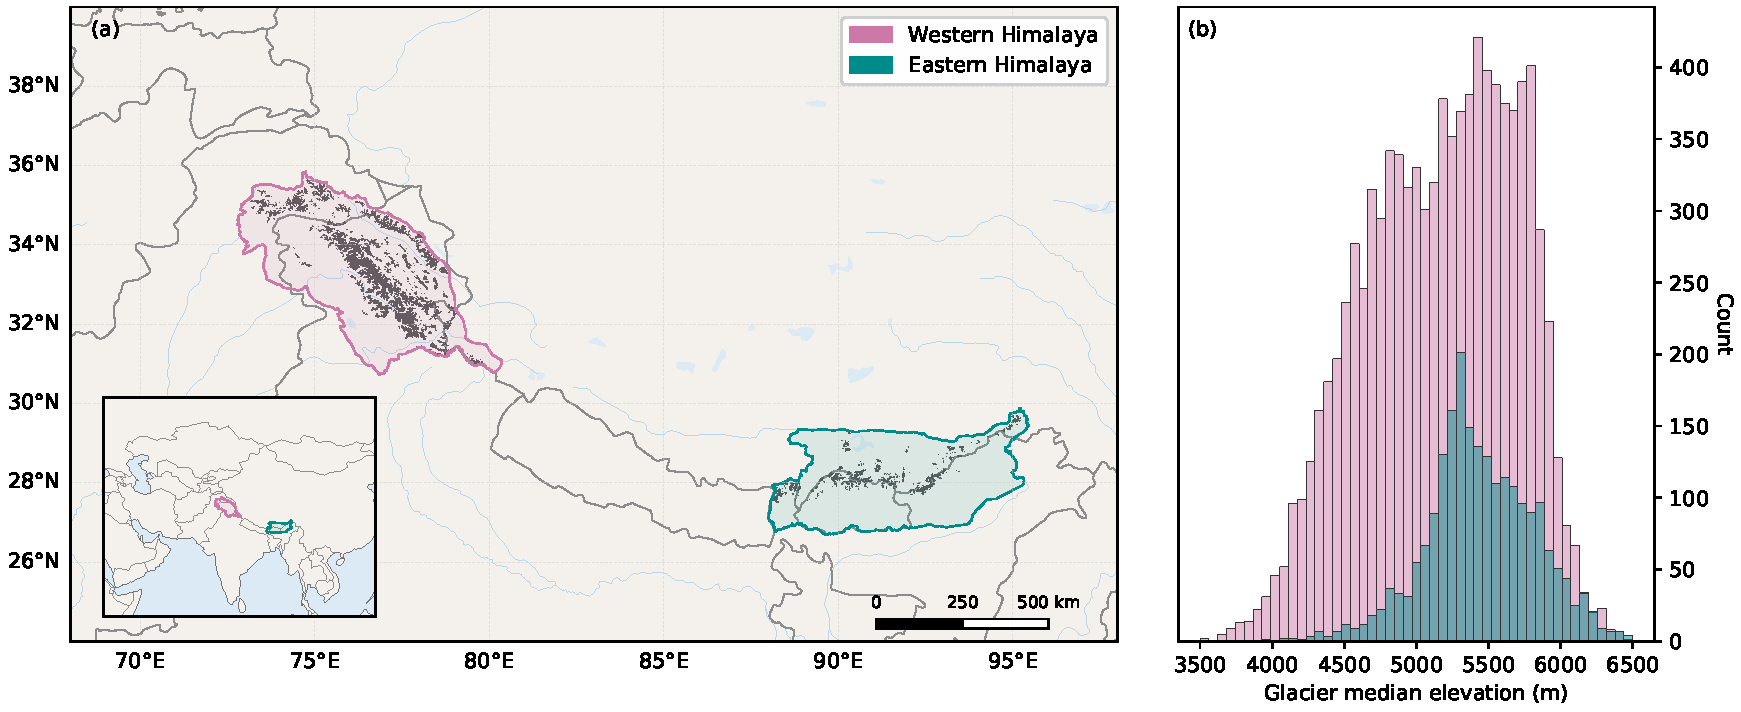
\includegraphics[width=\textwidth,height=.62\textheight,keepaspectratio]{fig01_study_area.pdf}\caption{Study regions and glacier elevations in High Mountain Asia. (a) Western and Eastern Himalayan domains defined by HIMAP (Bolch et al., 2019), with RGI v6.0 glacier outlines and an inset locating the domains within High Mountain Asia. (b) Distributions of RGI median glacier elevation for glacier population displayed in (a). The map shows all 11,685 study glaciers in the training, validation, and test groups, including the test glacier excluded from performance summaries.}\label{fig:study}\end{figure}

\FloatBarrier

\section{Data}
The Western and Eastern Himalaya are selected to examine how each method's performance varies in areas with different glacierized areas, glacier-wide characteristics, and regional surface elevation-change distributions (Figs.~\ref{fig:study} and \ref{fig:distributions}; Table~\ref{tab:metadata}). The two regions also differ in their climatic influences, with a greater contribution from winter westerly disturbances in the west and predominantly summer monsoon precipitation in the east \citep{bolch2019}. The availability of a common surface elevation-change product for both regions allows the methods to be compared using consistently processed reference data \citep{shean2020}. Regional extents follow the Hindu Kush Himalayan Monitoring and Assessment Programme (HIMAP; \citealp{bolch2019}). Figure~\ref{fig:study} shows the study domains and distributions of inventory median glacier elevation.

Surface elevation-change rates for 2000--2018 are taken from the 30\,m product distributed by \citet{sheands2020}. The underlying assessment combines ASTER and high-resolution WorldView/GeoEye stereo DEMs \citep{shean2020}. We use finite reference values within the retained glacier masks to create artificial voids and evaluate their reconstruction. These values provide a common reference for comparing methods, although they contain observational errors.

\begin{table}[!htbp]\centering\small
\caption{Glacier characteristics by region and data group. Area is the mean RGI inventory area (km$^2$). Elevation (m) and elevation-change rate (m a$^{-1}$) are reported as the mean ± standard deviation of individual glacier means. Each glacier mean is calculated from its reference pixels with finite elevation and elevation-change values prior to any masking. These glacier means receive equal weight, regardless of glacier size. Test rows describe the evaluated glaciers, excluding RGI60-14.17287.}\label{tab:metadata}
\begin{tabular}{llrrr}\toprule Region & Group & Mean area (km$^2$) & Elevation (m) & Elevation change (m a$^{-1}$)\\\midrule
 \multirow{3}{*}{Western Himalaya} & Train & 0.726 & 5186 $\pm$ 508 & -0.230 $\pm$ 0.313 \\
 & Validation & 0.791 & 5180 $\pm$ 504 & -0.242 $\pm$ 0.328 \\
 & Test & 0.736 & 5184 $\pm$ 505 & -0.234 $\pm$ 0.315 \\
 \midrule
\multirow{3}{*}{Eastern Himalaya}  & Train & 0.657 & 5442 $\pm$ 397 & -0.563 $\pm$ 0.487 \\
 & Validation & 0.654 & 5456 $\pm$ 392 & -0.569 $\pm$ 0.436 \\
 & Test & 0.619 & 5435 $\pm$ 372 & -0.557 $\pm$ 0.463 \\
 \bottomrule\end{tabular}\end{table}

\FloatBarrier

To efficiently handle the large spatial extent while preserving pixel-level resolution, the dataset is stored as a chunked raster data cube. The cube is divided into fixed-size spatial chunks, allowing individual glacier subsets to be accessed without loading the full domain into memory. Input layers are aligned to the exact 30\,m grid of the elevation-change raster in its Albers equal-area projection. Copernicus GLO-30 surface elevations \citep{opentopography2021} are aligned by bilinear resampling. Slope and aspect rasters are derived from the unmasked DEM prior to glacier extraction, avoiding artificial terrain artifacts at glacier-mask boundaries. 

Input datasets and their roles are summarized in Table~\ref{tab:data}.

\begin{table}[!htbp]\centering\small
\caption{Input datasets and roles. }\label{tab:data}
\begin{tabularx}{\textwidth}{p{.22\textwidth}p{.32\textwidth}X}\toprule
Input & Source & Role \\\midrule
Elevation-change rate & Shean (2020); Shean et al. (2020) & 2000--2018 reference and available observations; 30 m grid. \\
Surface elevation & Copernicus GLO-30; OpenTopography (2021) & Elevation; slope and aspect derived on aligned DEM. \\
Glacier outlines & RGI Consortium (2017), v6.0 & Support and glacier attributes. \\
Regional boundaries & HIMAP; Bolch et al. (2019) & Study domains and clipping assessment. \\
Lake-terminating inventory & \citet{luo2026} & 2022 polygon intersection filter. \\
Surge inventory and flags & \citet{guo2023}; RGI v6.0 & Interior-point match in any inventory class or RGI Surging flag 1--3. \\
\bottomrule\end{tabularx}\end{table}

\FloatBarrier

Glacier outlines were constructed by merging RGI v6.0 regions 13--15 \citep{rgi2017} and clipping to the Western and Eastern Himalayan HIMAP domains. Lake-terminating and surge-type glaciers were excluded to limit the influence of calving-related retreat and rapid ice redistribution. These processes can produce elevation-change patterns that differ from those of other glaciers, although their exclusion does not imply that retained elevation changes solely reflect surface mass balance. Of the 12,644 outlines in the study domains, 650 lake-terminating glaciers \citep{luo2026} and 34 surge-type glaciers \citep{guo2023} were removed from the dataset. An additional 276 glaciers were excluded due to incompatible geometries ($<50$ available pixels or domain boundary-edge artifacts). The final dataset contains 11,684 glaciers (Table~\ref{tab:population}).

\begin{figure}[!htbp]\centering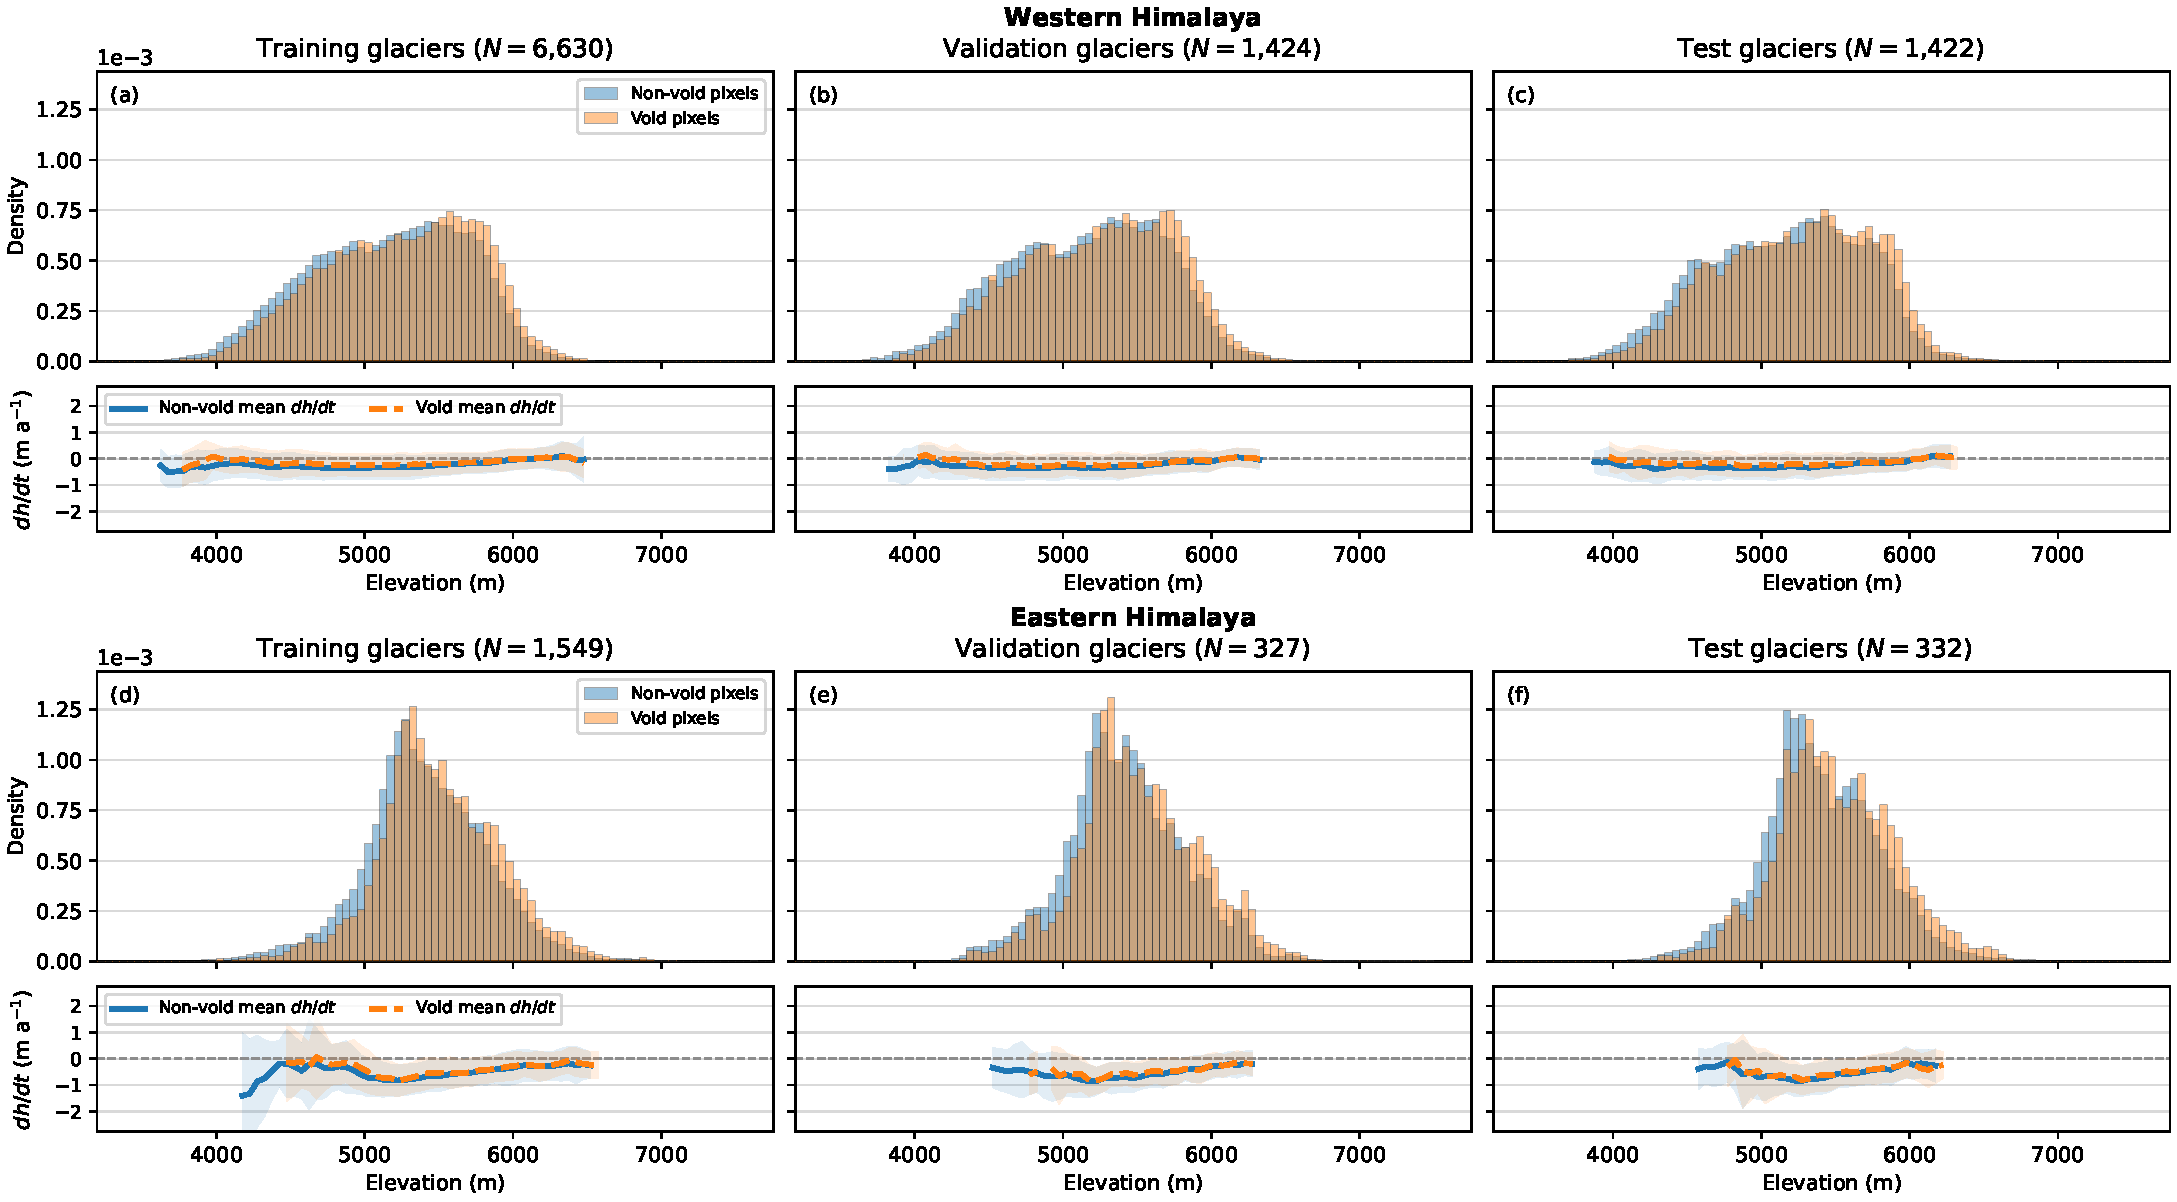
\includegraphics[width=\textwidth,height=.62\textheight,keepaspectratio]{fig02_distributions.pdf}\caption{Observed and withheld reference data in the Western (a–c) and Eastern (d–f) Himalaya, with columns showing training, validation, and test glaciers. Each lettered panel contains an elevation-density histogram above and elevation-change rates below. Blue denotes non-void pixels available to the methods, and orange denotes withheld void pixels. Histograms use 50 m elevation bins. Curves show bin-mean reference elevation-change rates for 2000–2018, with shading indicating within-bin standard deviations. Glaciers receive equal total weight, with equal weights for realizations and then finite pixels within each realization. Membership is defined separately for each mask. Training and validation panels show all 8,179 and 1,751 assigned glaciers. Test panels show the 1,754 evaluated test glaciers, excluding RGI60-14.17287. All panels share one elevation range spanning every finite reference pixel, from 3,195 to 7,755 m.}\label{fig:distributions}\end{figure}

\FloatBarrier

Throughout the analysis, ``glacier-wide'' refers to the valid reference support within the retained raster masks, with area calculated from the valid-pixel count. The Western Himalaya contains substantially more retained glaciers than the Eastern Himalaya, and the two regions have different glacier elevation and elevation-change distributions (Table~\ref{tab:metadata}; Fig.~\ref{fig:distributions}). The distribution of mean elevation-change rates also differs with elevation. These regional summaries describe the reference data and the observations available under artificial masking but do not distinguish physical variation from reference-product error.

\begin{table}[!htbp]\centering\small
\caption{Glacier population counts and elevation-change data coverage by region and dataset group. Reference-data area is the number of glacier pixels with finite reference elevation-change values multiplied by 900 m$^2$. Pixel counts and reference-data areas are reported before artificial masking. Test-performance summaries exclude RGI60-14.17287 and its five void realizations, leaving 1,422 Western and 332 Eastern glaciers for evaluation. The assigned Western test group has 1,423 glaciers, 1,239,146 reference pixels, and 1,115.23 km$^2$ of reference-data area.}\label{tab:population}
\begin{tabular}{llrrr}\toprule
Region & Group & $N$ Glaciers & $N$ Reference pixels & Reference-data area (km$^2$)\\\midrule
\multirow{3}{*}{Western Himalaya} & Training & 6,630 & 5,304,156 & 4,773.74\\
 & Validation & 1,424 & 1,242,677 & 1,118.41\\
 & Test & 1,422 & 1,153,251 & 1,037.93\\\midrule
\multirow{3}{*}{Eastern Himalaya} & Training & 1,549 & 1,081,312 & 973.18\\
 & Validation & 327 & 227,774 & 205.00\\
 & Test & 332 & 218,490 & 196.64\\
\bottomrule\end{tabular}\end{table}

\FloatBarrier


\section{Methods}

\subsection{Artificial void generation}
Artificial voids allow the methods to be evaluated against withheld reference elevation-change values. Here, void geometry refers to the spatial configuration of a mask, including its area fraction, shape, and position within the glacier elevation range. Voids in historical DEMs are variable, frequently contiguous, and often concentrated in glacier accumulation zones. We use contiguous, elevation-biased masks to approximate these characteristics under controlled conditions, without assuming that they reproduce every process responsible for real missing data. 

For each glacier, five artificial-void realizations are retained to evaluate performance across different void configurations. Five was a practical choice rather than a number determined by a convergence criterion, and the sensitivity to this choice is examined using subsets of the retained realizations (Fig.~\ref{fig:realizations}). A realization refers to one mask which is processed independently. The five masks are not combined into a single larger void. They may overlap, and a pixel hidden in one realization can be available in another. The void fraction (expressed as a fraction of the glacier's valid reference area) for each realization was determined via sampling from a truncated normal distribution with a mean of 0.37 and standard deviation of 0.08, bounded between 0.15 and 0.60 of the eligible glacier pixels. This methodology aims to represent the variability present in void size and geometry in real data while matching the mean void size reported in \citet{maurer2019}.

Each mask starts from an eligible seed pixel at or above the glacier's median eligible elevation and grows through an eight-neighbor flood-fill algorithm \citep{newman1979} until the requested pixel count is reached or no connected eligible pixels remain. Neighbor exploration is randomized and void growth can extend below the median elevation, meaning that the seed restriction does not confine the entire void to the upper half of the glacier. The five masks provide repeated configurations for each glacier, not independent glacier observations. Diagnostic statistics were computed for each void realization to quantify metrics such as the void fraction of reference glacier area, the number of void pixels, the fraction of upper-half elevation pixels designated as void, and the elevation offset between void pixels and the full glacier distribution. The results of this void-generation workflow are stored in a chip file for each glacier, containing the glacier mask, a void mask for each realization, along with coordinates, elevation, and elevation-change values for each pixel. In addition, the diagnostic statistics are reported for each realization across all glaciers in a single metadata table.
 
We refer to glacier pixels with finite elevation-change values in the original dataset as reference pixels. For each artificial-void realization, these pixels are divided into observed pixels, whose values remain available for reconstruction, and withheld pixels, whose values are hidden and used as training labels or evaluation targets. These definitions are formalized using the following notation. For glacier $g$ and realization $r$, let $G_g$ denote the set of reference pixels and $V_{g,r}$ denote the set of withheld artificial-void pixels. The observed pixels are defined as \(O_{g,r}=G_g\cap V_{g,r}^{\prime}\), where $V_{g,r}^{\prime}$ denotes the complement of the withheld pixel set.

\subsection{Glacier partitioning and spatial structure}

Glaciers are assigned to training, validation, and test groups in an approximate 70:15:15 ratio, with all pixels and void realizations from each glacier kept in the same group (Table~\ref{tab:population}). For model development, a subset of the training glaciers is further divided using square spatial blocks with a width of 100\,km. Each selected block is assigned to one of the following roles: model fitting, hyperparameter tuning, or confirmation. Glaciers selected from that block can contribute only to its assigned role, giving 598 glaciers for fitting, 199 for tuning, and 200 for confirmation. No block contributes glaciers to more than one development subset. This block assignment applies only to model development as the overall training, validation, and test groups remain partitioned by glacier and may contain neighboring glaciers with correlated signals or measurement errors. Spatial-block resampling of test performance is described in Sect.~\ref{sec:bootstrap}.

\subsection{Constant void-filling: local mean}
The most straightforward void-filling approach assigns a single value to all void pixels within a glacier based on the mean surface elevation-change rate of the available pixels from that glacier. For each glacier and realization,
\begin{equation}
\widehat y^{\mathrm{con}}_{g,r,i}=\frac{1}{|O_{g,r}|}\sum_{j\in O_{g,r}}y_{g,j},\qquad i\in V_{g,r},
\end{equation}
where $y$ denotes the reference elevation-change rate. The mean is recalculated for every realization, so it can change with void size and placement. The method assumes spatially uniform elevation change within the void and serves as a baseline for evaluating more sophisticated techniques. Among constant-filling approaches, only the local mean method is evaluated in this study, given the findings of \citet{mcnabb2019}.

\subsection{Hypsometric void-filling: local elevation-bin mean}
We implement a hypsometric approach to account for elevation-dependent variations in glacier surface change. Following the local elevation-bin framework evaluated by \citet{mcnabb2019}, available pixels are grouped into 50\,m elevation bins where glacier relief is at least 500\,m, and into ten equally spaced bins otherwise. Bin limits are defined from the finite on-glacier DEM elevations, including the elevations of void pixels. The mean reference elevation-change rate in each occupied bin is calculated using only $O_{g,r}$. A void pixel receives the mean elevation-change value for its elevation bin.
An elevation bin can contain known elevations but no available elevation-change observations. If all bins are occupied, their means are used directly. Otherwise, missing-bin means are estimated using a third-degree polynomial fitted to the occupied-bin means when at least four bins are occupied and the observed elevation span covers at least two-thirds of the glacier elevation range. Occupied-bin means are retained. In other cases, missing-bin means are estimated by linear interpolation between occupied bin centers, with constant extension of the nearest occupied-bin value outside their range. If only one bin is occupied, its mean is used for the missing bins. Thus, empty bins beyond the observed range require extrapolation, even though their surface elevations are known. The resulting realization-specific hypsometric void-filling estimate is denoted $\widehat y^{\mathrm{hyp}}_{g,r,i}$.


\subsection{Machine learning void-filling: hybrid hypsometric--machine learning}

We implement a machine learning approach using gradient-boosted decision tree regression, XGBoost \citep{chen2016}, to estimate surface elevation change across void areas. Rather than directly predicting elevation change, the model is trained to estimate the departure between a reference value and its realization-specific hypsometric baseline:
\begin{equation}
d_{g,r,i}=y_{g,i}-\widehat y^{\mathrm{hyp}}_{g,r,i},\qquad
\widehat y^{\mathrm{xgb}}_{g,r,i}=\widehat y^{\mathrm{hyp}}_{g,r,i}+f(\mathbf X_{g,r,i}).
\label{eq:target}
\end{equation}
Here, $d$ is the hypsometric departure and serves as the training target, $f(\mathbf X)$ is the predicted hypsometric departure, and $\widehat y-y$ is the reconstruction error used to compare methods. This formulation retains the hypsometric estimate while allowing the model to represent deviations from it and does not impose a physical constraint on those deviations. A single model is trained using glaciers from both regions. Absolute and glacier-relative coordinates, along with glacier and realization identifiers, are excluded from its predictors. Projected coordinates are used to calculate distances and spatial blocks, but are not supplied directly to the learner. The final predictor set contains nine static attributes and 16 context variables (Table~\ref{tab:features}).

\subsubsection{Model predictors}
The static predictors describe pixel elevation, slope and aspect, together with glacier area, minimum, median and maximum elevation, and hypsometric index. Elevation represents gradients associated with temperature and other environmental conditions; it is not itself a complete physical explanation of elevation change. Slope is a pixel-level terrain derivative. Aspect is represented by dimensionless sine and cosine components of azimuth measured clockwise from north.

Context predictors describe the observations available in each realization. They include the hypsometric estimate, the number and fraction of observations in the target elevation bin, observed-bin variability, whether the bin is empty, whether the target lies beyond the observed elevation range, the observed elevation span, and the void fraction. They also describe distance to available observations and local departures from the hypsometric relationship. All elevation-change summaries are recomputed after masking $V_{g,r}$.

The local-departure predictor uses up to 32 available source pixels from the same glacier and realization, strictly within 900\,m of the target. At source pixel $j$, the departure is $y_{g,j}-\widehat y^{\mathrm{hyp}}_{g,r,j}$. Their distance-weighted mean is
\begin{equation}
L_{g,r,i}=\frac{\sum_{j\in S_{g,r,i}}\exp\!\left(-\frac{\ell_{ij}}{300\,\mathrm m}\right)(y_{g,j}-\widehat y^{\mathrm{hyp}}_{g,r,j})}{\sum_{j\in S_{g,r,i}}\exp\!\left(-\frac{\ell_{ij}}{300\,\mathrm m}\right)},
\end{equation}
where $\ell_{ij}$ is projected distance and $S_{g,r,i}$ contains the selected sources. When fewer than three sources are available, the predictor is assigned a missing value. Native missing-value handling is retained for undefined context quantities. Only available observations enter these predictors.

\begin{table*}[t]
\caption{Predictors used in the hybrid XGBoost model. The model uses nine static glacier and terrain predictors and 16 additional predictors describing the hypsometric baseline, elevation, and observations remaining in each realization.}
\label{tab:features}
\centering
\small
\begin{tabular}{p{0.22\textwidth}p{0.29\textwidth}p{0.40\textwidth}}
\tophline
Description & Variable(s) & Description \\
\middlehline
\multicolumn{3}{l}{Static glacier and terrain predictors (9)} \\
\middlehline
\rowcolor[gray]{0.94}
Elevation & $z$ & Pixel DEM elevation (m). \\

Slope & $slope$ & Pixel slope calculated using the Horn operator (degrees). \\

\rowcolor[gray]{0.94}
Aspect components & $aspect_{\sin}$, $aspect_{\cos}$ & Sine and cosine of pixel aspect; dimensionless. \\

Glacier area & $Area_g$ & Inventory glacier area (km$^2$). \\

\rowcolor[gray]{0.94}
Inventory elevations & $Zmin_g$, $Zmed_g$, $Zmax_g$ & Minimum, median, and maximum glacier elevation (m). \\

Hypsometric index & $HI_g$ & Inventory-derived hypsometric index; dimensionless. \\
\middlehline
\multicolumn{3}{l}{Additional predictors (16)} \\
\middlehline
\rowcolor[gray]{0.94}
Hypsometric estimate & $hyp$ & Realization-specific estimate $\widehat y^{\mathrm{hyp}}$ (m a$^{-1}$). \\

Normalized elevation &$z_{norm}$ & $(z-Z_{\mathrm{min}})/(Z_{\mathrm{max}}-Z_{\mathrm{min}})$, using inventory elevation limits. \\
\rowcolor[gray]{0.94}
Band source count & $band\_count$ & Number of observed source pixels in the target elevation bin. \\

Band source fraction & $band\_frac$ & Source count divided by the number of glacier pixels with finite elevation in that bin. \\
\rowcolor[gray]{0.94}
Band variability & $band\_std$ & Sample standard deviation of observed source values in the bin (m a$^{-1}$). \\

Empty band & $band\_empty$ & Indicator that the bin contains no observed source pixels. \\

\rowcolor[gray]{0.94}
Outside observed elevations & $out\_obs\_z$ & Indicator that target elevation lies outside the observed source elevation range. \\

Nearest occupied band & $nearest\_band\_dz$ & Elevation difference to the nearest occupied bin center (m). \\

\rowcolor[gray]{0.94}
Observed elevation span & $\textit{obs\_span\_frac}$ & Observed source elevation range divided by the elevation range of glacier pixels with finite elevation. \\

Void fraction & $void\_frac$ & Fraction of glacier pixels with finite elevation that lie within the artificial-void mask. \\

\rowcolor[gray]{0.94}
Band-fill indicators & \textit{mode\_none}, \textit{mode\_cubic}, \textit{mode\_linear} & Three binary indicators identifying the hypsometric missing-bin rule. \\

Nearest observation & \textit{nearest\_source\_m} & Distance to the nearest observed source pixel (m), without the 900 m cutoff. \\

\rowcolor[gray]{0.94}
Local source count & \textit{local\_count} & Number of selected source pixels strictly within 900 m, capped at 32. \\

Local hypsometric departure & \textit{local\_residual} & Distance-weighted mean source departure, $L$ (m a$^{-1}$). \\
\bottomhline
\end{tabular}
\end{table*}

\FloatBarrier

\subsubsection{Hyperparameter optimization and training}
Training examples are artificial-void targets on training glaciers. Their predictors are calculated from the observations remaining in the same realization. For $R_g$ void realizations and $N_{g,r}=|V_{g,r}|$ target pixels, weights defined as
\begin{equation}
w_{g,r,i}=\frac{1}{R_gN_{g,r}},
\end{equation}
and normalized to a mean of one during fitting. This gives each glacier equal total weight, distributed equally across its realizations and then across their target pixels. The learner minimizes weighted squared error in $d$, equivalent to weighted squared reconstruction error when $\widehat y^{\mathrm{hyp}}$ is fixed.

Hyperparameter optimization uses Optuna's tree-structured Parzen estimator \citep{akiba2019} with sampler seed 42. The development-fitting set contains 506,629 rows after capping targets at 500 per glacier--realization. The tuning and confirmation sets contain 312,003 and 379,672 targets, respectively. We run 100 trials for the hybrid model and 100 for a static-predictor residual control, for 200 trials in total. The control uses the same target and baseline but only the nine static predictors. Each trial uses histogram-based XGBoost training with at most 2,000 boosting rounds and early stopping after 50 rounds without improvement in tuning-set glacier-balanced pixel root mean square error (RMSE). The selected model parameters minimize this RMSE.

The selected configurations are locked before confirmation-set prediction and checked using seeds 42--44. The final hybrid model uses squared-error regression, a histogram maximum bin count of 256, learning rate 0.02337, maximum depth 5, minimum child weight 23.7263, row subsampling 0.62927, column subsampling 0.60414, minimum split loss 1.58038, L1 regularization $7.29\times10^{-8}$, and L2 regularization 9.26169. It is fitted once at seed 42 with 172 trees on all 11,792,199 training targets. Search ranges and development diagnostics accompany the archived model outputs.

\subsection{Reconstruction errors and glacier-wide estimates}
Pixel-scale evaluation is restricted to common artificial-void targets. For each method, $m$, reconstruction error is
\begin{equation}
	e_{m,g,r,i}=\widehat y_{m,g,r,i}-y_{g,i}
\end{equation}
where positive errors indicate a more positive reconstructed rate. Pixel mean absolute error (MAE), RMSE, and bias use weights $1/(|\mathcal G|R_gN_{g,r})$, where $\mathcal G$ is the evaluated glacier group. Pixel normalized median absolute deviation (NMAD) is 1.4826 times the weighted median absolute deviation about the weighted median error. These are glacier-balanced metrics, not pooled pixel statistics. Non-void pixels are not added as zero-error observations.

To compare the original and reconstructed glacier-wide signals directly, let $a=900\,\mathrm{m^2}$ and $A_g=a|G_g|$. Thus, the reference ($\dot V^{\mathrm{ref}}$) and reconstructed ($\dot V^{\mathrm{rec}}$) volume-change rates are defined by the following equations:
\begin{align}
\dot V_g^{\mathrm{ref}}=a\sum_{i\in G_g}y_{g,i}, \qquad
\dot V_{m,g,r}^{\mathrm{rec}}=a\left(\sum_{i\in O_{g,r}}y_{g,i}+\sum_{i\in V_{g,r}}\widehat y_{m,g,r,i}\right).
\end{align}

The glacier-wide specific error ($E$) is
\begin{equation}
E_{m,g,r}=\frac{\dot V_{m,g,r}^{\mathrm{rec}}-\dot V_g^{\mathrm{ref}}}{A_g}
=\frac{1}{|G_g|}\sum_{i\in V_{g,r}}e_{m,g,r,i}.
\label{eq:glacier}
\end{equation}
We compare four estimates: the reference and the constant, hypsometric, and hybrid reconstructions. Observed non-void values are retained in each reconstruction, and their contributions cancel in the reconstruction error. This property means the error in glacier-wide volume-change rate equals the void-integrated error. Glacier MAE is the mean of $|E_{m,g,r}|$ over realizations and then glaciers, RMSE is the square root of the correspondingly averaged $E_{m,g,r}^2$, and bias is the signed average of $E_{m,g,r}$. Glacier NMAD is calculated from each glacier's mean signed error across realizations. Integrated-error metrics use the same aggregation with $a\sum_{i\in V_{g,r}}e_{m,g,r,i}$ in place of $E_{m,g,r}$. Integrated quantities have units of \volrate; no density conversion to mass balance is applied. All retained test glacier--realizations have predictions covering their complete artificial void. The denominator $A_g$ is valid reference area rather than void area or total inventory area.

\subsection{Spatial-block intervals for aggregate performance}\label{sec:bootstrap}
We estimate uncertainty in aggregate reconstruction performance using a paired spatial-block bootstrap. Glaciers are assigned to square blocks by the projected centroid of their retained raster mask. Whole blocks are sampled with replacement within each region, keeping every glacier and all its realizations together. The same block draw is used for all methods. We use 2,000 draws and report the 2.5th and 97.5th percentiles as 95\% intervals. The primary block width is 100 km, with 50 and 200 km used to examine sensitivity. The Western and Eastern test populations occupy 24 and 15 blocks at 100 km, respectively, decreasing to nine and six at 200 km.

Figure \ref{fig:bootstrap} compares methods using paired differences, such that $\Delta M=M_{\mathrm{comparison}}-M_{\mathrm{baseline}}$. Negative differences indicate lower error for the comparison method. For bias, we subtract the magnitudes of the population mean signed errors, so negative differences indicate smaller bias magnitude. Signed biases are reported separately in the performance tables.

Percentage reductions in the Results and Figure \ref{fig:relative} are calculated by dividing the baseline-minus-comparison difference by the baseline value and multiplying by 100. Positive percentages indicate lower error for the comparison method. Relative bias reductions are omitted because baseline biases close to zero make these ratios unstable.

Contrasts and percentage reductions are recalculated within each paired bootstrap draw. Pixel NMAD point estimates are exact, while its bootstrap intervals use resampled weighted block histograms. These intervals describe aggregate performance uncertainty conditional on the fitted model and evaluated sample. They do not include retraining variability or quantify predictive uncertainty for an individual void.

\subsection{Spatial examples, elevation bands, and realization sensitivity}\label{sec:diagnostics}
Four test glaciers, two per region, were selected using metadata and void geometry before examining their reconstruction errors. The examples show the five retained masks and, for one realization, the reference, observed, reconstruction, and target-only errors (Figs.~\ref{fig:masks} and \ref{fig:examples}). Figure~\ref{fig:masks} shows the five retained masks for one glacier per region while Fig.~\ref{fig:examples} shows reconstruction examples for four test glaciers.”These analyses illustrate behavior and are not a representative performance sample.

Using each glacier's saved hypsometric bin edges, we decompose reference variance into within- and between-bin terms (Fig.~\ref{fig:bands}). Separately for each realization, observed-minus-withheld mean and standard-deviation contrasts are calculated for bins with at least three observed and three withheld pixels. Bin contrasts are weighted by withheld pixel counts within a realization, then averaged over realizations and equally over glaciers. Coverage fractions use the same realization-then-glacier aggregation. Error summaries for occupied and empty observed bins are conditional on the relevant bin rather than representing overall metrics calculated across all withheld pixels.

We evaluate every nonempty subset of the five realizations (31 subsets), applying the same subset to each method. For each glacier, we compare subset MAE and the hybrid-minus-hypsometric ranking with their five-realization values. The sign-disagreement fraction averages over subsets and then glaciers. Regional sensitivity envelopes use 1,000 random subset selections; they describe mask sensitivity, not confidence intervals. Geometry summaries use achieved void-fraction and mean normalized void-elevation tertiles selected without model-error information (Fig.~\ref{fig:realizations}). Mean normalized void elevation is the average of $(z_i-z_g^{\min})/(z_g^{\max}-z_g^{\min})$ over the void targets, where $z_g^{\min}$ and $z_g^{\max}$ are the elevation limits of the glacier raster support.

\subsection{Regional transfer and coordinate ablation}\label{sec:sensitivities}
Two supplementary experiments assess different aspects of geographic sensitivity. For regional transfer, 1,000 original-training glaciers per region were selected by metadata, using 100 km block quotas and within-block coverage of area and median elevation. A 100 km separation rule from the other region's test outlines removed no source glaciers. Each source-region model uses at most 200 targets per realization, the fixed model settings and 172 rounds, and is evaluated on both regions' complete test targets (Table~\ref{tab:transfer}; Fig.~\ref{fig:transfer}). Local observations on target glaciers remain available to construct their hypsometric and context predictors; this is not prediction for an entirely unobserved region.

The coordinate experiment combines those two source samples into one shared set of 2,000 training glaciers and 1,128,098 rows. Two models are fitted from scratch with identical rows, labels, weights, seed and fixed settings: the 25 accepted predictors, and the same 25 plus absolute projected pixel-center easting and northing. Training weights give each glacier equal contribution; thus the balanced source sample gives the regions equal total training weight. Both models use 172 rounds without additional tuning or early stopping. The full-data model uses all 8,179 training glaciers, whereas this experiment compares two models fitted on the same capped sample. Both fits use the same column-subsampling fraction (Table~\ref{tab:coordinates}; Fig.~\ref{fig:coordinates}).

Both experiments use paired 100 km whole-block intervals with 2,000 draws and retain all realizations per glacier. Coordinate contrasts are coordinates-off minus coordinates-on; positive error-magnitude contrasts favor inclusion. Combined coordinate intervals resample within both regions. The fixed settings are shared between the experiments; each feature set is not optimized separately.


\section{Results}

All three methods are evaluated on the same 2,540,722 artificial-void target pixels from 1,754 test glaciers and 8,770 glacier--realizations. These test-performance summaries exclude RGI60-14.17287 and its five realizations. This post hoc evaluation exclusion does not change the training data, fitted models, glacier split, void masks, or saved predictions. A pixel appearing in several realizations is counted once in each relevant realization. Metrics are reported to three significant figures, and percentage changes are calculated from unrounded values.

\subsection{Pixel-scale performance}
Constant filling has pixel MAEs of 0.265\,\rate\ in the Western Himalaya and 0.367\,\rate\ in the Eastern Himalaya (Fig.~\ref{fig:residuals}; Table~\ref{tab:pixel}). Hypsometric MAE is 5.99\% and 3.68\% lower, respectively. Hybrid MAE is 21.4\% and 17.8\% lower than constant MAE and 16.4\% and 14.7\% lower than hypsometric MAE. NMAD follows the same method ordering.

\begin{figure}[!htbp]\centering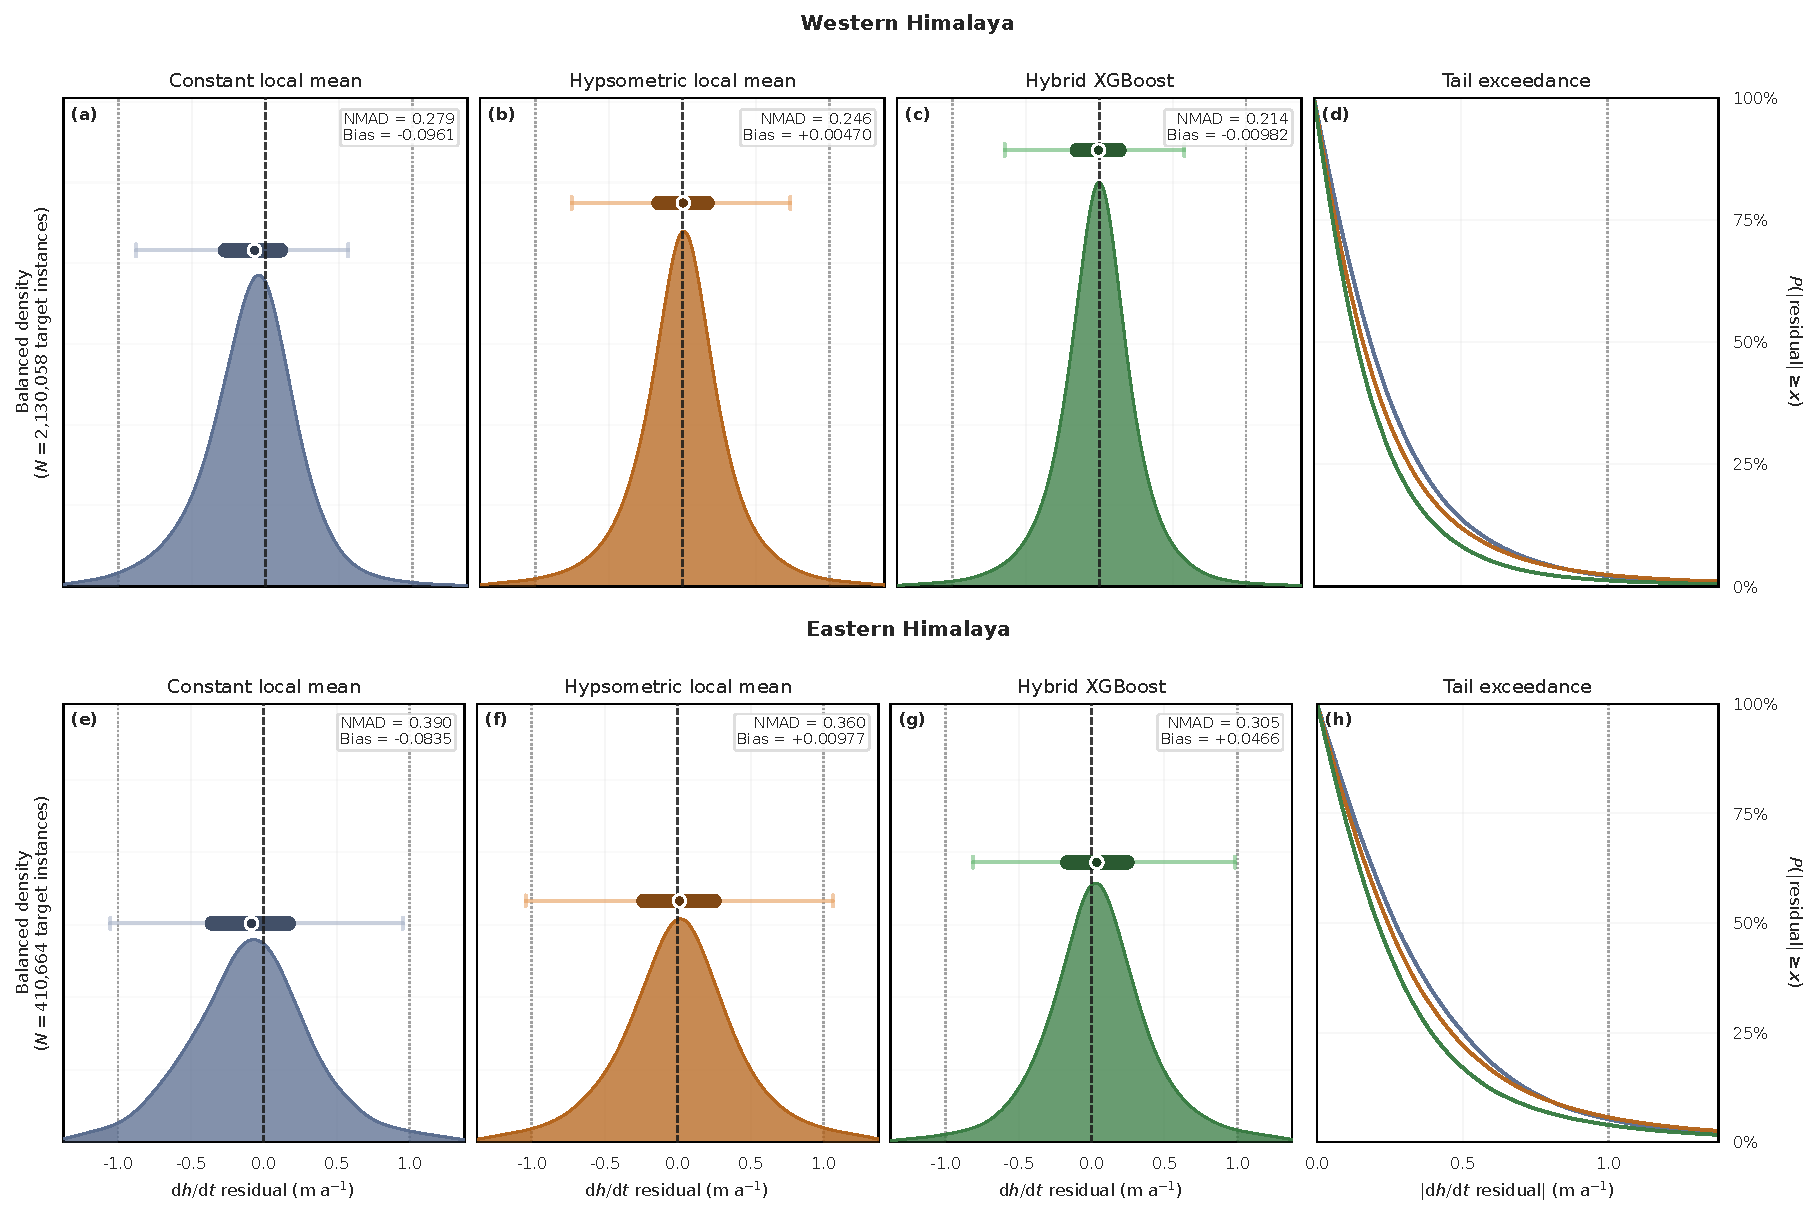
\includegraphics[width=\textwidth,height=.62\textheight,keepaspectratio]{fig03_pixel_residuals.pdf}\caption{Glacier-balanced pixel reconstruction errors for constant, hypsometric, and hybrid void-filling in the Western (a–c) and Eastern (e–g) Himalaya. Error is predicted minus reference elevation-change rate on identical withheld targets. Smoothed densities use a common vertical scale. White circles mark weighted medians, thick bars span the interquartile range, and thin whiskers span the 2.5th–97.5th percentiles. Panels (d,h) show the weighted probability that absolute error equals or exceeds the horizontal-axis value. Glaciers receive equal total weight, with equal weights for realizations and then target pixels. Counts refer to target instances across realizations, from 1,422 Western and 332 Eastern evaluated test glaciers.}\label{fig:residuals}\end{figure}


\FloatBarrier


\begin{table}[!htbp]
\centering\small
\setlength{\tabcolsep}{5pt}
\caption{Glacier-balanced pixel reconstruction errors on identical withheld targets (m a$^{-1}$). Each glacier receives equal total weight, divided equally among its realizations and then their target pixels. Bias is predicted minus reference elevation-change rate. Western and Eastern counts are 2,130,058 and 410,664 target instances.}
\label{tab:pixel}
\begin{tabular}{llrrrr}
\toprule
Region & Method & MAE & RMSE & NMAD & Bias \\
\midrule
Western & Constant & $0.265$ & $0.372$ & $0.279$ & $-0.0961$ \\
 & Hypsometric & $0.249$ & $0.388$ & $0.246$ & {\boldmath$+0.00470$} \\
 & Hybrid & {\boldmath$0.208$} & {\boldmath$0.310$} & {\boldmath$0.214$} & $-0.00982$ \\
\midrule
Eastern & Constant & $0.367$ & $0.517$ & $0.390$ & $-0.0835$ \\
 & Hypsometric & $0.353$ & $0.524$ & $0.360$ & {\boldmath$+0.00977$} \\
 & Hybrid & {\boldmath$0.301$} & {\boldmath$0.446$} & {\boldmath$0.305$} & $+0.0466$ \\
\midrule
Combined & Constant & $0.284$ & $0.403$ & $0.296$ & $-0.0937$ \\
 & Hypsometric & $0.269$ & $0.417$ & $0.264$ & $+0.00566$ \\
 & Hybrid & {\boldmath$0.226$} & {\boldmath$0.340$} & {\boldmath$0.228$} & {\boldmath$+0.000864$} \\
\bottomrule
\end{tabular}
\belowtable{Evaluation excludes RGI60-14.17287 and its five realizations. Western, Eastern, and combined counts are 1,422, 332, and 1,754 glaciers. Values are rounded to three significant figures. Bold identifies the lowest error metric and the bias closest to zero within each population, using unrounded values.}
\end{table}

\FloatBarrier

Hypsometric RMSE is slightly higher than constant RMSE in both regions, whereas hybrid RMSE is lower than both. Constant void-filling has negative signed bias in both regions while hypsometric filling has the smallest absolute regional biases. The hybrid bias values are between those of the two baselines in both regions. For the combined summary, the opposite-signed Western and Eastern hybrid biases partly cancel, resulting in a small bias magnitude. At 100\,km block width, the paired pixel-MAE interval for hypsometric-minus-constant filling is below zero in the west and spans zero in the east. Hybrid-minus-constant and hybrid-minus-hypsometric intervals are below zero in both regions (Fig.~\ref{fig:bootstrap}; Table~\ref{tab:paired}).

\begin{figure}[!htbp]\centering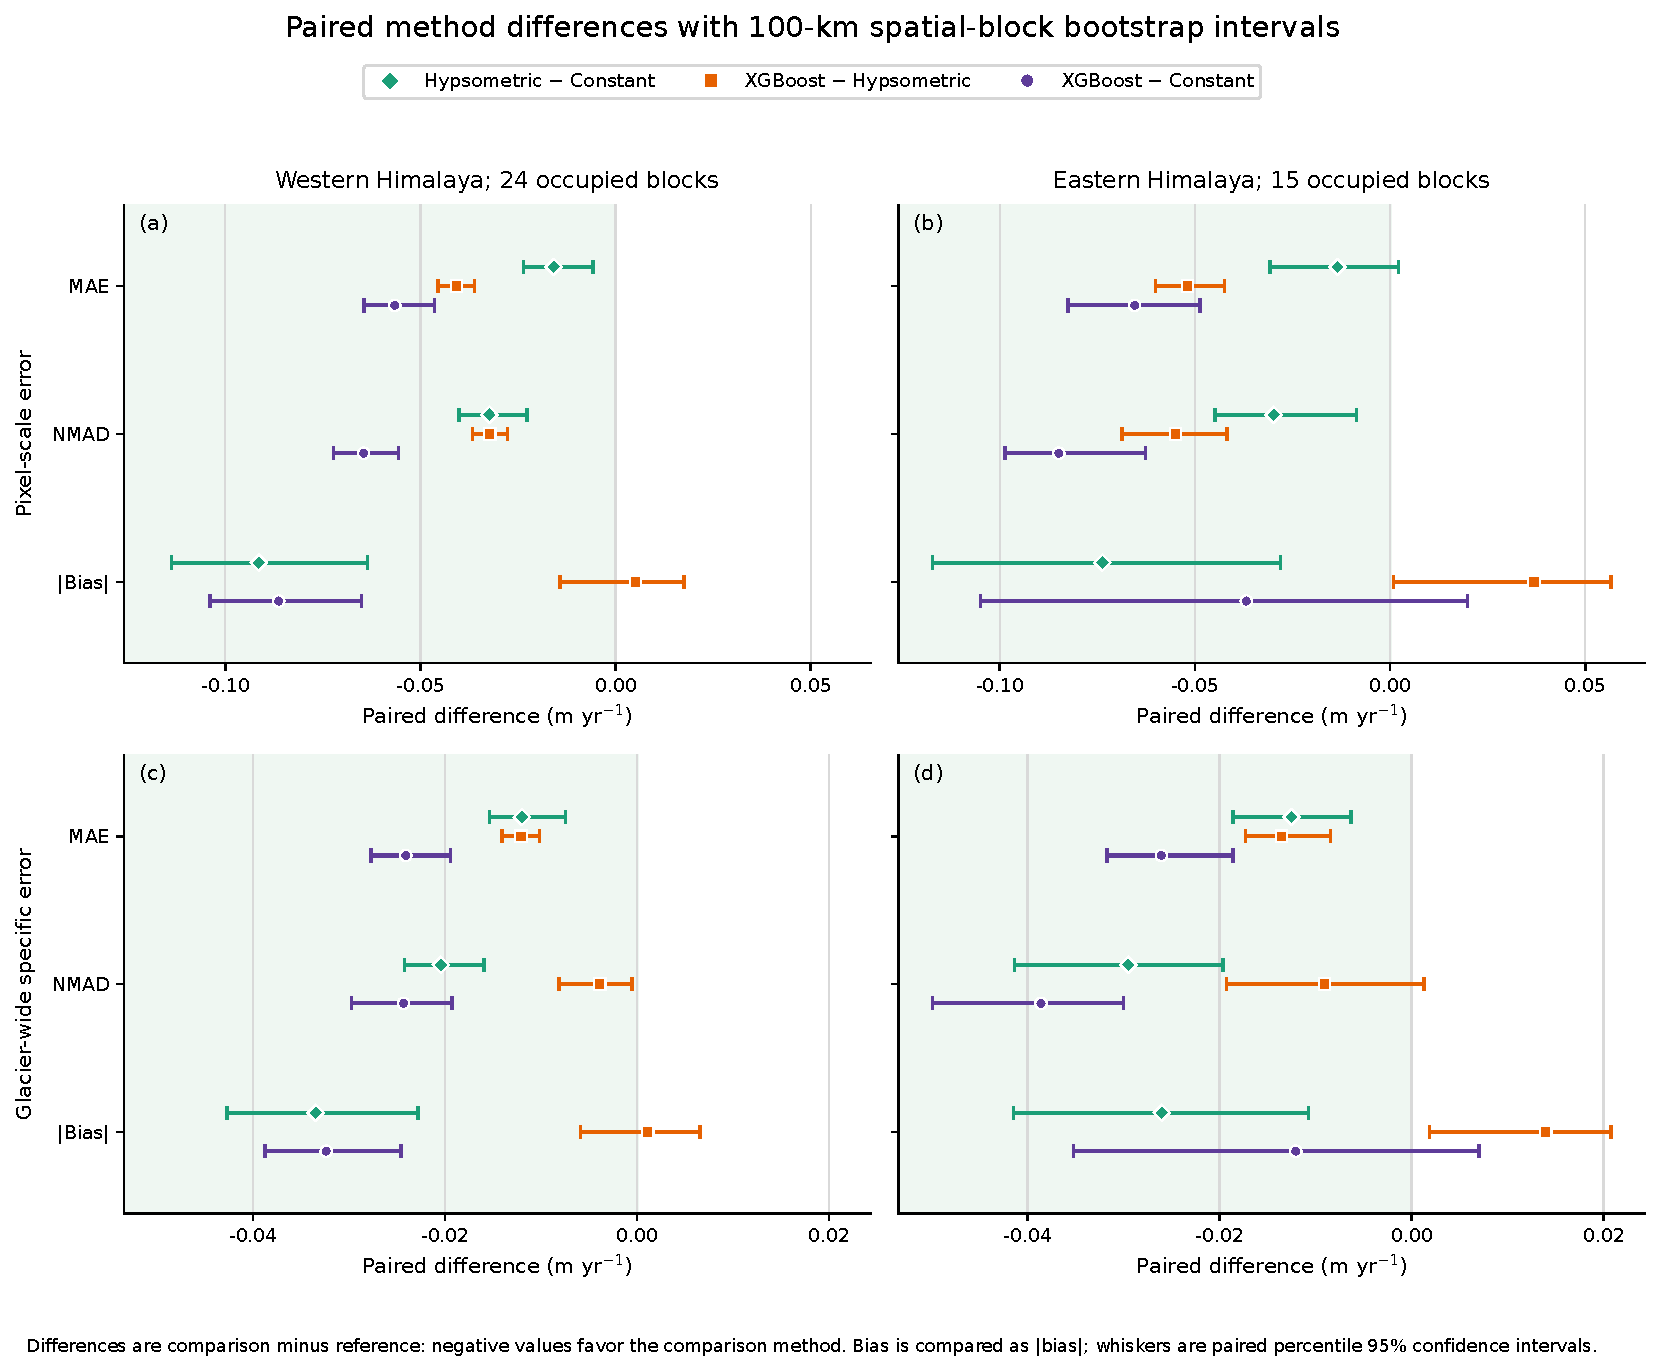
\includegraphics[width=\textwidth,height=.62\textheight,keepaspectratio]{fig04_bootstrap_contrasts.pdf}\caption{Paired method contrasts for pixel errors (a,b) and glacier-wide specific errors (c,d) in the Western (left) and Eastern (right) Himalaya. Symbols show comparison-minus-baseline differences in MAE, NMAD, and absolute bias for the three method pairs identified in the legend. Negative values indicate a lower error metric for the comparison method. Bias contrasts subtract the magnitudes of population mean signed errors. Bars show 95\% percentile intervals from 2,000 paired spatial-block bootstrap draws using 100 km blocks, with all realizations of each glacier retained together. The evaluated test population excludes RGI60-14.17287.}\label{fig:bootstrap}\end{figure}


\FloatBarrier


\begin{table}[!htbp]
\centering\small
\setlength{\tabcolsep}{5pt}
\caption{Hybrid-minus-hypsometric error contrasts with 95\% percentile intervals in brackets (m a$^{-1}$). Intervals use 2,000 paired spatial-block draws with 100\,km blocks. Negative values favor hybrid filling. Bias contrasts subtract the magnitudes of population mean signed errors.}
\label{tab:paired}
\begin{tabular}{lrr}
\toprule
Metric & Western & Eastern \\
\midrule
Pixel MAE & $-0.0407\,[-0.0455, -0.0362]$ & $-0.0519\,[-0.0601, -0.0425]$ \\
Pixel absolute bias & $+0.00512\,[-0.0143, +0.0175]$ & $+0.0368\,[+0.000805, +0.0565]$ \\
Glacier MAE & $-0.0121\,[-0.0141, -0.0101]$ & $-0.0136\,[-0.0173, -0.00845]$ \\
Glacier NMAD & $-0.00389\,[-0.00812, -0.000519]$ & $-0.00909\,[-0.0193, +0.00127]$ \\
Glacier absolute bias & $+0.00111\,[-0.00588, +0.00654]$ & $+0.0140\,[+0.00184, +0.0207]$ \\
\bottomrule
\end{tabular}
\belowtable{Evaluation excludes RGI60-14.17287 and its five realizations. Western, Eastern, and combined counts are 1,422, 332, and 1,754 glaciers. Values are rounded to three significant figures. Point estimates and interval endpoints are rounded independently.}
\end{table}

\FloatBarrier


\subsection{Glacier-wide elevation and volume-change reconstruction}
The constant void-filling method has glacier-wide specific-error MAEs of 0.0721\,\rate\ for the Western Himalaya and 0.0927\,\rate\ in the Eastern Himalaya (Table~\ref{tab:glacier}; Fig.~\ref{fig:glacier}). Hypsometric MAE is 16.6\% and 13.5\% lower, respectively. The hybrid method's MAE is lower than both baselines and reduces MAE by 20.1\% and 16.9\% relative to hypsometric void-filling. The combined hybrid MAE is 0.0515\,\rate, 32.2\% below constant MAE and 19.4\% below hypsometric MAE. The hybrid method's MAE is lower than the hypsometric method's for 1,224 of 1,754 test glaciers (69.8\%).

\begin{table}[!htbp]
\centering\small
\setlength{\tabcolsep}{5pt}
\caption{Glacier-wide specific reconstruction errors over valid reference-data area (m a$^{-1}$). Absolute, squared, and signed errors are averaged over realizations and then equally over glaciers to calculate MAE, RMSE, and bias. RMSE is the square root of the averaged squared error. NMAD is calculated across glacier-mean signed errors.}
\label{tab:glacier}
\begin{tabular}{llrrrr}
\toprule
Region & Method & MAE & RMSE & NMAD & Bias \\
\midrule
Western & Constant & $0.0721$ & $0.101$ & $0.0614$ & $-0.0357$ \\
 & Hypsometric & $0.0601$ & $0.0942$ & $0.0410$ & {\boldmath$+0.00223$} \\
 & Hybrid & {\boldmath$0.0480$} & {\boldmath$0.0713$} & {\boldmath$0.0371$} & $-0.00333$ \\
\midrule
Eastern & Constant & $0.0927$ & $0.125$ & $0.0852$ & $-0.0303$ \\
 & Hypsometric & $0.0802$ & $0.116$ & $0.0557$ & {\boldmath$+0.00423$} \\
 & Hybrid & {\boldmath$0.0666$} & {\boldmath$0.0961$} & {\boldmath$0.0466$} & $+0.0182$ \\
\midrule
Combined & Constant & $0.0760$ & $0.106$ & $0.0660$ & $-0.0347$ \\
 & Hypsometric & $0.0639$ & $0.0987$ & $0.0432$ & $+0.00261$ \\
 & Hybrid & {\boldmath$0.0515$} & {\boldmath$0.0766$} & {\boldmath$0.0385$} & {\boldmath$+0.000741$} \\
\bottomrule
\end{tabular}
\belowtable{Evaluation excludes RGI60-14.17287 and its five realizations. Western, Eastern, and combined counts are 1,422, 332, and 1,754 glaciers. Values are rounded to three significant figures. Bold identifies the lowest error metric and the bias closest to zero within each population, using unrounded values.}
\end{table}

\FloatBarrier

Hypsometric filling has the smallest absolute glacier-wide biases in both regions, followed by hybrid and constant filling. The hybrid-minus-hypsometric absolute-bias contrast is positive in the east, with a 100 km interval excluding zero. The corresponding Western contrast and the Eastern glacier-NMAD contrast have intervals spanning zero (Table~\ref{tab:paired}).

\begin{figure}[!htbp]\centering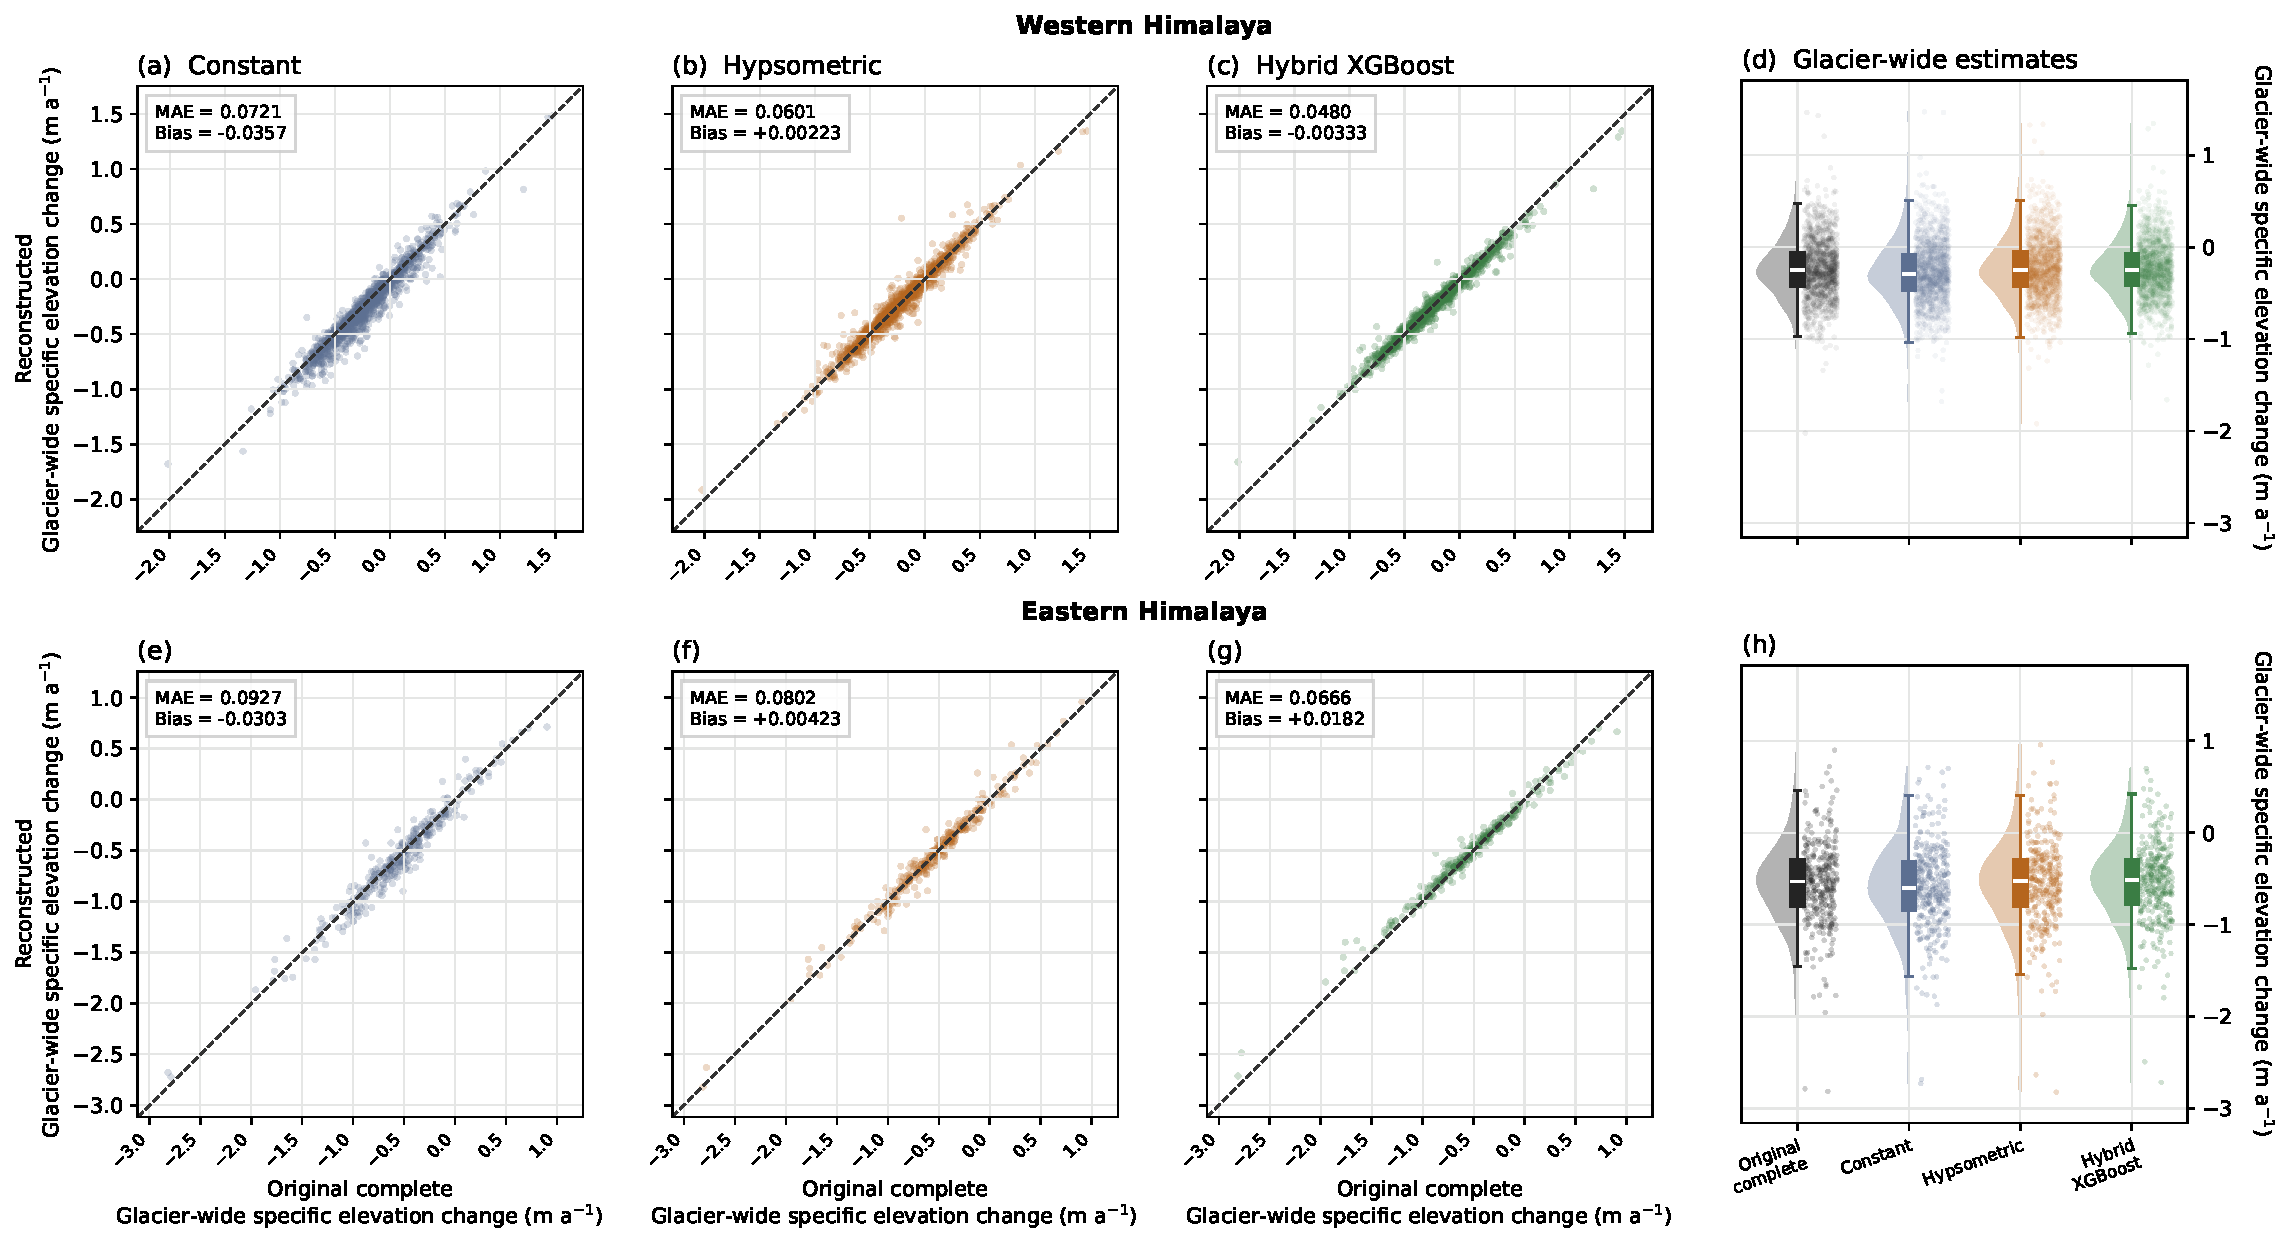
\includegraphics[width=\textwidth,height=.62\textheight,keepaspectratio]{fig05_glacier_wide.pdf}\caption{Reconstructed versus reference glacier-wide specific elevation-change rates for constant, hypsometric, and hybrid filling in the Western (a–c) and Eastern (e–g) Himalaya. Each point represents one of the 1,754 evaluated test glaciers, with reconstructed rates averaged over its five realizations. Dashed diagonals indicate equality. Panels (d,h) combine smoothed distributions, individual glacier points, and boxes showing medians and interquartile ranges. Whiskers extend to the most extreme values within 1.5 interquartile ranges of each box. Observed non-void values are retained in each reconstruction. “Original complete” denotes the available reference-data area before artificial void generation.}\label{fig:glacier}\end{figure}


Per-glacier integrated volume-rate MAE follows the same constant, hypsometric, and hybrid ordering in both regions (Table~\ref{tab:volume}). Hypsometric MAE is 33.1\% and 31.9\% below constant MAE in the Western and Eastern Himalaya, respectively. The hybrid MAE is a further 19.8\% and 16.1\% lower than the hypsometric MAE. Hybrid integrated RMSE is lower than both baselines in both regions, with reductions of 6.03\% in the Western Himalaya and 9.76\% in the Eastern Himalaya relative to the hypsometric method. For the combined-domain, the hybrid method's integrated RMSE is $1.87\times 10^{5}$ \volrate, 6.20\% lower than the hypsometric method's RMSE.

\begin{table}[!htbp]
\centering\small
\setlength{\tabcolsep}{5pt}
\caption{Per-glacier integrated volume-rate reconstruction errors (m$^3$ a$^{-1}$). Each error equals glacier-wide specific error multiplied by valid reference-data area. Metrics give equal weight to realizations within each glacier and equal weight to glaciers within each population. Observed values are retained, so reconstruction error arises entirely from withheld pixels.}
\label{tab:volume}
\begin{tabular}{llrrr}
\toprule
Region & Method & MAE & RMSE & Bias \\
\midrule
Western & Constant & $6.81\times10^{4}$ & $3.81\times10^{5}$ & $-3.76\times10^{4}$ \\
 & Hypsometric & $4.55\times10^{4}$ & $2.17\times10^{5}$ & {\boldmath$+4.13\times10^{3}$} \\
 & Hybrid & {\boldmath$3.65\times10^{4}$} & {\boldmath$2.04\times10^{5}$} & $+4.92\times10^{3}$ \\
\midrule
Eastern & Constant & $6.04\times10^{4}$ & $1.84\times10^{5}$ & $-4.01\times10^{4}$ \\
 & Hypsometric & $4.11\times10^{4}$ & $9.95\times10^{4}$ & $-7.99\times10^{3}$ \\
 & Hybrid & {\boldmath$3.45\times10^{4}$} & {\boldmath$8.98\times10^{4}$} & {\boldmath$+5.81\times10^{3}$} \\
\midrule
Combined & Constant & $6.66\times10^{4}$ & $3.52\times10^{5}$ & $-3.81\times10^{4}$ \\
 & Hypsometric & $4.47\times10^{4}$ & $2.00\times10^{5}$ & {\boldmath$+1.83\times10^{3}$} \\
 & Hybrid & {\boldmath$3.62\times10^{4}$} & {\boldmath$1.87\times10^{5}$} & $+5.09\times10^{3}$ \\
\bottomrule
\end{tabular}
\belowtable{Evaluation excludes RGI60-14.17287 and its five realizations. Western, Eastern, and combined counts are 1,422, 332, and 1,754 glaciers. Values are rounded to three significant figures. Bold identifies the lowest error metric and the bias closest to zero within each population, using unrounded values.}
\end{table}

\FloatBarrier

\subsection{Spatial, elevation-band, and realization diagnostics}

The spatial examples show variation in method rankings among glaciers and error metrics (Figs.~\ref{fig:masks} and \ref{fig:examples}). In the four geometry-selected examples, hypsometric and hybrid filling both have lower void-target MAE and absolute glacier-specific error than constant filling. Hybrid void-target MAE is lower than hypsometric MAE in three cases and 15.2\% higher in the fourth, while its absolute glacier-specific error is lower in only one.

On an equal-glacier average, 53.0\% of Western and 55.5\% of Eastern Himalaya reference variance lies within elevation bands (Fig.~\ref{fig:bands}). In eligible bins, observed-minus-withheld mean contrasts are $+0.004$ and $+0.018$\,\rate, with intervals spanning zero, while absolute local contrasts average 0.179 and 0.257\,\rate. Observed-bin standard deviations exceed withheld-bin standard deviations in both regions. Empty observed bins contain an average of 14.3\% and 13.7\% of withheld targets, respectively, using realization-then-glacier averaging.

Within bins containing observations, the constant method's MAE exceeds hypsometric MAE, and hybrid MAE is lower than both. In empty observed bins, hypsometric MAE instead exceeds constant MAE by 19.7\% in the west and 16.2\% in the east. Hybrid MAE remains below both, with reductions relative to hypsometric filling of 30.2\% and 24.9\%. Eastern empty-bin signed errors are negative for hypsometric filling and positive for hybrid filling.

The constant, hypsometric, and hybrid MAE ordering persists across the realization-subset sensitivity envelopes and each void-geometry group (Fig.~\ref{fig:realizations}). However, hypsometric MAE is lower than hybrid MAE in 25.5\% of Western and 25.2\% of Eastern Himalaya comparisons based on a single realization. All methods have higher glacier-wide specific-error MAE in the largest void-fraction group than in the smallest. 

\subsection{Regional transfer and coordinate sensitivity}
Both same-region and cross-region hybrid models have lower glacier-wide specific MAE than the constant and hypsometric baselines (Table~\ref{tab:transfer}). Cross-region training increases MAE relative to same-region training by 17.0\% in the Western Himalaya and 10.8\% in the Eastern Himalaya, with paired difference intervals above zero. Integrated volume-rate RMSE increases by 72.5\% in the Western Himalaya but decreases by 2.58\% in the Eastern Himalaya.

\begin{table}[!htbp]
\centering\small
\setlength{\tabcolsep}{5pt}
\caption{Regional-transfer performance on common test targets. Glacier MAE and signed bias are in m a$^{-1}$. Integrated RMSE describes per-glacier volume-rate errors in m$^3$ a$^{-1}$. Each regional hybrid uses 1,000 source glaciers. The full-data hybrid uses all 8,179 training glaciers from both regions.}
\label{tab:transfer}
\begin{tabular}{llrrr}
\toprule
Target & Model & Glacier MAE & Bias & Integrated RMSE \\
\midrule
Western & Constant & $0.0721$ & $-0.0357$ & $3.81\times10^{5}$ \\
 & Hypsometric & $0.0601$ & $+0.00223$ & $2.17\times10^{5}$ \\
 & Hybrid (full data) & {\boldmath$0.0480$} & $-0.00333$ & $2.04\times10^{5}$ \\
 & Hybrid (Western-trained) & $0.0488$ & {\boldmath$+0.00121$} & {\boldmath$1.55\times10^{5}$} \\
 & Hybrid (Eastern-trained) & $0.0571$ & $-0.0280$ & $2.67\times10^{5}$ \\
\midrule
Eastern & Constant & $0.0927$ & $-0.0303$ & $1.84\times10^{5}$ \\
 & Hypsometric & $0.0802$ & $+0.00423$ & $9.95\times10^{4}$ \\
 & Hybrid (full data) & $0.0666$ & $+0.0182$ & $8.98\times10^{4}$ \\
 & Hybrid (Western-trained) & $0.0737$ & $+0.0358$ & {\boldmath$8.78\times10^{4}$} \\
 & Hybrid (Eastern-trained) & {\boldmath$0.0665$} & {\boldmath$-0.00343$} & $9.02\times10^{4}$ \\
\bottomrule
\end{tabular}
\belowtable{Evaluation excludes RGI60-14.17287 and its five realizations. Western, Eastern, and combined counts are 1,422, 332, and 1,754 glaciers. Values are rounded to three significant figures. Bold identifies the lowest error metric and the bias closest to zero within each population, using unrounded values.}
\end{table}

\FloatBarrier

In the matched coordinate experiment, including absolute projected coordinates reduces glacier-wide specific MAE by 1.23\% in the west, 1.48\% in the east, and 1.29\% across the combined sample (Fig.~\ref{fig:coordinateintervals}; Table~\ref{tab:coordinates}). Paired 95\% spatial-block intervals for the off-minus-on MAE contrasts are above zero in both regions and the combined sample. Glacier-wide specific bias magnitudes decrease by 84.1\%, 88.5\%, and 83.3\%, respectively. The absolute-bias contrast intervals exclude zero in the Western and combined samples but span zero in the east.

Coordinate inclusion produces smaller reductions in per-glacier integrated volume-rate RMSE, at 0.0292\% in the Western Himalaya, 0.255\% in the Eastern Himalaya, and 0.0405\% across the combined sample. Integrated volume-rate bias magnitudes increase by 120\%, 458\%, and 37.9\%, respectively. The paired integrated MAE, RMSE, and absolute-bias contrast intervals span zero in each region and the combined sample.

\begin{table}[!htbp]
\centering\small
\setlength{\tabcolsep}{5pt}
\caption{Matched hybrid models with absolute projected coordinates excluded (off) or included (on), alongside constant and hypsometric baselines. The off model uses 25 predictors, and the on model adds projected pixel-center easting and northing. Both models use identical capped training rows, labels, weights, seed, and fixed settings. MAE and Bias describe glacier-wide specific errors in m a$^{-1}$. Vol. RMSE and Vol. bias describe per-glacier integrated volume-rate errors in m$^3$ a$^{-1}$. Biases are signed.}
\label{tab:coordinates}
\begin{tabular}{llrrrr}
\toprule
Region & Method / arm & MAE & Bias & Vol. RMSE & Vol. bias \\
\midrule
Western & Constant & $0.0721$ & $-0.0357$ & $3.81\times10^{5}$ & $-3.76\times10^{4}$ \\
 & Hypsometric & $0.0601$ & $+0.00223$ & $2.17\times10^{5}$ & $+4.13\times10^{3}$ \\
 & Hybrid (coords off) & $0.0493$ & $-0.0105$ & $1.78\times10^{5}$ & {\boldmath$-1.66\times10^{3}$} \\
 & Hybrid (coords on) & {\boldmath$0.0487$} & {\boldmath$-0.00166$} & {\boldmath$1.78\times10^{5}$} & $+3.65\times10^{3}$ \\
\midrule
Eastern & Constant & $0.0927$ & $-0.0303$ & $1.84\times10^{5}$ & $-4.01\times10^{4}$ \\
 & Hypsometric & $0.0802$ & $+0.00423$ & $9.95\times10^{4}$ & $-7.99\times10^{3}$ \\
 & Hybrid (coords off) & $0.0656$ & $+0.00721$ & $8.44\times10^{4}$ & {\boldmath$-8.36\times10^{2}$} \\
 & Hybrid (coords on) & {\boldmath$0.0646$} & {\boldmath$+0.000832$} & {\boldmath$8.42\times10^{4}$} & $-4.66\times10^{3}$ \\
\midrule
Combined & Constant & $0.0760$ & $-0.0347$ & $3.52\times10^{5}$ & $-3.81\times10^{4}$ \\
 & Hypsometric & $0.0639$ & $+0.00261$ & $2.00\times10^{5}$ & $+1.83\times10^{3}$ \\
 & Hybrid (coords off) & $0.0524$ & $-0.00711$ & $1.64\times10^{5}$ & {\boldmath$-1.50\times10^{3}$} \\
 & Hybrid (coords on) & {\boldmath$0.0517$} & {\boldmath$-0.00119$} & {\boldmath$1.64\times10^{5}$} & $+2.07\times10^{3}$ \\
\bottomrule
\end{tabular}
\belowtable{Evaluation excludes RGI60-14.17287 and its five realizations. Western, Eastern, and combined counts are 1,422, 332, and 1,754 glaciers. Values are rounded to three significant figures. Bold identifies the lowest error metric and the bias closest to zero within each population, using unrounded values.}
\end{table}

\FloatBarrier


\section{Discussion}
The three void-filling methods examined in this study differ in how they represent elevation-change patterns and use the observations remaining around a void. The constant method, which estimates a mean value from all available observations, is sensitive to sparsely represented elevation bands. Since higher areas of a glacier's surface tend to thin less rapidly, the preferential removal of high-elevation observations during the artificial void generation process results in a more negative observed mean. This provides a plausible explanation for the negative constant-method biases when evaluated using the elevation-biased voids (Fig.~\ref{fig:distributions}).

Hypsometric void-filling represents the elevation gradient present in glacier surface elevation change. This method estimates individual band means from fewer observations since each band only uses the in-band values. Therefore, sparse sampling, local extremes, and extrapolation into unobserved bands can offset its advantage over the glacier-wide constant method. This trade-off helps explain why hypsometric filling reduces MAE and bias without consistently reducing pixel RMSE. Observation coverage and the representativeness of retained values matter alongside the strength of the elevation-change relationship \citep{mcnabb2019}.

The hybrid void-filling method uses observed hypsometric departures and glacier attributes to adjust the band estimate. Nearby departures may describe spatial patterns that elevation alone cannot distinguish, while targets farther from observations depend more strongly on relationships learned across glaciers. However, within-band variability includes both physical variation and reference-product error, so its magnitude does not establish how much physical signal the hybrid method recovers or provide a lower bound on glacier-wide error since opposing pixel errors can cancel during spatial averaging.

The larger errors present in the Eastern Himalaya across all methods may reflect differences in target variability, observation coverage, and reference quality. Eastern Himalayan glaciers exhibit more negative and variable mean elevation-change rates across elevations and a broader distribution of glacier-mean elevation change rates, as compared to glaciers in the Western Himalaya (Fig.~\ref{fig:distributions}; Table~\ref{tab:metadata}). These differences could make Eastern Himalayan reconstructions more sensitive to how well observations represent the elevation-change pattern across a void. Differences in accumulation, melt, glacier geometry, and ice redistribution could also alter elevation gradients and spatial departures from band means \citep{bolch2019, shean2020}.

The combined-domain hybrid model may encounter different predictor–departure relationships in the two regions. Western glaciers contribute more total fitting weight because they are more numerous, despite equal weighting of individual glaciers. Incomplete representation of Eastern Himalaya conditions could therefore contribute to the hybrid method's positive bias and larger error. The matched coordinate experiment suggests that location contains information relevant to the mean correction to some degree but does not fully correct the error. It cannot establish that training imbalance or coordinate omission causes the full model’s Eastern bias.


Each error metric analyzed in this study emphasizes a different property of reconstruction. Smaller absolute errors can coexist with a shift in the signed mean, while RMSE gives greater influence to occasional large errors. The training objective also minimizes glacier-balanced squared pixel errors rather than glacier-wide specific MAE or integrated volume-rate RMSE. Better pixel predictions therefore need not produce the best glacier-wide integral. Opposing errors can cancel during averaging while spatially coherent errors can persist \citep{rolstad2009,hugonnet2022}.

At the pixel scale, the hybrid method’s lower NMAD in both regions indicates a tighter central spread of reconstruction errors, complementing its lower MAE and RMSE. Hypsometric filling also reduces NMAD relative to constant filling while increasing RMSE, consistent with a narrower central distribution but greater influence from large deviations. This pattern could reflect sensitivity to sparse observations or extrapolation in particular elevation bands.

Integrated volume-rate error equals glacier-wide specific error multiplied by valid reference-data area. Consequently, each glacier’s contribution to the mean squared integrated error is its squared specific error multiplied by the square of its reference area. Integrated RMSE therefore gives greater influence to errors on larger glaciers. Although area scaling preserves comparisons of error magnitude between methods for an individual glacier, it can change their ordering across the evaluated sample. Specific and integrated summaries thus provide complementary measures of reconstruction performance, with the preferred method depending on the error characteristic of interest.

The coordinate experiment also illustrates why specific and integrated biases can respond differently. Moving the mean specific error closer to zero does not necessarily improve cancellation among area-scaled signed errors. Large relative increases in integrated bias partly reflect small starting bias magnitudes and do not imply comparable increases in typical glacier error. Paired confidence intervals spanning zero further limit the evidence for changes in integrated performance. Similarly, opposite-signed regional errors can produce a small combined bias while masking larger biases within each region.

The increase in MAE under cross-region training suggests that learned departure relationships are not fully transferable between the two regions. The differing responses of MAE and integrated RMSE are consistent with changes in how errors are distributed across glaciers and glacier sizes. Local observations remain available on target glaciers, so these experiments assess transfer of the learned correction while retaining target-specific context.

The modest MAE benefit from including coordinates in the hybrid model indicates that absolute location supplies information beyond the accepted terrain and context predictors under the matched experimental settings. Coordinates could represent climatic structure, glacier characteristics, or spatially correlated reference errors. Coordinate inclusion can bring glacier-wide specific bias closer to zero while increasing integrated bias magnitude if the corrections cancel less effectively after errors are scaled by glacier area. The large relative increases in integrated bias partly reflect small initial bias magnitudes, while the paired intervals spanning zero limit evidence for a consistent deterioration in integrated performance.

The choice to include coordinates may depend on the intended application. For reconstruction within the sampled geographic domain, coordinate inclusion offers a modest advantage when glacier-wide specific MAE is the primary criterion. Excluding coordinates may be appropriate when limiting direct reliance on location-specific relationships is a priority. For applications prioritizing per-glacier integrated volume-rate errors, the paired intervals provide no clear basis for preferring either configuration.

Spatial-block intervals describe aggregate performance uncertainty conditional on the fitted models. They do not remove training–test dependence or include variability from refitting and model selection. Coarser blocks also leave fewer units for resampling, limiting interval stability. Individual predictive uncertainty remains unresolved because prediction-minus-reference errors combine reconstruction and reference-product errors. Separating these components and propagating uncertainty through glacier-wide reconstructions requires compatible reference-error information and explicit treatment of spatial covariance  \citep{hugonnet2022}.

Repeated masks reveal sensitivity to which observations remain, rather than providing independent glacier samples. Stable population-level ordering can therefore coexist with unstable individual-glacier rankings. Larger voids remove both target values and contextual information, but comparisons among the lower, middle, and upper thirds of the void-geometry distribution involve different glacier mixtures and do not isolate a causal effect of void size. The overlapping masks also share one reference field, so the subset analysis cannot establish convergence beyond the retained realizations.

Historical applications introduce changes in observation period, glacier state, resolution, and error structure that can alter both the hypsometric relationship and the usefulness of local context. The modern calibration therefore requires separate validation before transfer. Tests with masks derived from actual image matching and independent observation periods would provide more direct evidence of applicability \citep{mcnabb2019}. Evaluation also remains limited to the reference-data area and retained glacier types; native gaps and entirely unobserved glaciers are not tested. Future development should prioritize spatially separated validation and calibrated prediction intervals across observation-coverage conditions.

\conclusions[Conclusions]
We compared constant, hypsometric, and hybrid hypsometric--machine learning void-filling methods using artificially generated voids on each of 1,754 test glaciers in the Western and Eastern Himalaya. Relative to the hypsometric method, the hybrid method reduces combined glacier-wide specific MAE by 19.4\%, from 0.0639 to 0.0515 \rate. Pixel MAE decreases by 16.4\% in the Western Himalaya and 14.7\% in the Eastern Himalaya, accompanied by lower pixel NMAD in both regions. Combined per-glacier integrated volume-rate RMSE decreases by 6.20\%, although this comparison is sensitive to large, influential glaciers. These findings support using glacier- and pixel-specific observational context to improve reconstruction beyond elevation-bin means.

These general improvements coincide with larger glacier-wide specific bias and increased sensitivity to geographic transfer and void geometry for Eastern Himalaya glaciers. Including absolute spatial coordinates reduces the combined-domain specific MAE by 1.29\% in the matched experiment, while its integrated-performance intervals provide no clear preference between configurations. Coordinate use should therefore reflect the intended application and error metric. Next steps should prioritize geographically separated model development and evaluation, together with tests using independent observation periods and void patterns derived from actual image matching. The analysis and quantification of calibrated predictive uncertainty for this method's reconstruction ability, specifically using a dataset with compatible reference-error information and directly addressing spatial covariance when combining pixel errors into glacier-wide estimates, should be prioritized in future work.

\clearpage

\codedataavailability{The reference elevation-change product is available from \citet{sheands2020}. The project code repository is \url{https://github.com/cmarkovsky/ensemble_void_fill}.}

\authorcontribution{CM and SR designed the study; CM developed and implemented the code for artificial void generation, void filling, analysis, and figure creation; CM wrote the manuscript, with all other authors contributing edits.}

\competinginterests{The authors declare that they have no conflict of interest.}

\begin{acknowledgements}
This work was funded by NASA HiMAT 19-HMA19-0029 and NASA 80NSSC22K1866, and NSF 2218664 and 1853881. We thank the University of Utah Center for High Performance Computing (CHPC) for computational resources and input on model design.
\end{acknowledgements}

\begin{thebibliography}{99}

\bibitem[Akiba et al.(2019)]{akiba2019} Akiba, T., Sano, S., Yanase, T., Ohta, T., and Koyama, M.: Optuna: A next-Generation Hyperparameter Optimization Framework, in: Proceedings of the 25th ACM SIGKDD International Conference on Knowledge Discovery \& Data Mining, Kdd ’19, pp. 2623–2631, Association for Computing Machinery, New York, NY, USA, ISBN 978-1-4503-6201-6, \url{https://doi.org/10.1145/3292500.3330701}, 2019.

\bibitem[Arendt et al.(2002)]{arendt2002} Arendt, A. A., Echelmeyer, K. A., Harrison, W. D., Lingle, C. S., and Valentine, V. B.: Rapid Wastage of Alaska Glaciers and Their Contribution to Rising Sea Level, Science, 297, 382–386, \url{https://doi.org/10.1126/science.1072497}, 2002.

\bibitem[Bamber and Rivera(2007)]{bamber2007} Bamber, JL. and Rivera, A.: A Review of Remote Sensing Methods for Glacier Mass Balance Determination, Global and Planetary Change, 59, 138–148, \url{https://doi.org/10.1016/j.gloplacha.2006.11.031}, 2007.

\bibitem[Berthier et al.(2023)]{berthier2023} Berthier, E., Floriciou, D., Gardner, A. S., Gourmelen, N., Jakob, L., Paul, F., Treichler, D., Wouters, B., Belart, J. M. C., Dehecq, A., Dussaillant, I., Hugonnet, R., Kääb, A., Krieger, L., Pálsson, F., and Zemp, M.: Measuring Glacier Mass Changes from Space—a Review, Reports on Progress in Physics, 86, 036 801, \url{https://doi.org/10.1088/1361-6633/acaf8e}, 2023.

\bibitem[Bhattacharya et al.(2021)]{bhattacharya2021} Bhattacharya, A., Bolch, T., Mukherjee, K., King, O., Menounos, B., Kapitsa, V., Neckel, N., Yang, W., and Yao, T.: High Mountain Asian glacier response to climate revealed by multi-temporal satellite observations since the 1960s, Nature Communications, 12, 4133, \url{https://doi.org/10.1038/s41467-021-24180-y}, 2021.

\bibitem[Bolch et al.(2011)]{bolch2011} Bolch, T., Pieczonka, T., and Benn, D. I.: Multi-decadal mass loss of glaciers in the Everest area (Nepal Himalaya) derived from stereo imagery, The Cryosphere, 5, 349–358, \url{https://doi.org/10.5194/tc-5-349-2011}, 2011.

\bibitem[Bolch et al.(2019)]{bolch2019} Bolch, T., Shea, J. M., Liu, S., Azam, F. M., Gao, Y., Gruber, S., Immerzeel, W. W., Kulkarni, A., Li, H., Tahir, A. A., Zhang, G., and Zhang, Y.: Status and Change of the Cryosphere in the Extended Hindu Kush Himalaya Region, in: The Hindu Kush Himalaya Assessment, edited by Wester, P., Mishra, A., Mukherji, A., and Shrestha, A. B., pp. 209–255, Springer International Publishing, Cham, ISBN 978-3-319- 92287-4 978-3-319-92288-1, \url{https://doi.org/10.1007/978-3-319-92288-1_7}, 2019.

\bibitem[Bolibar et al.(2020)]{bolibar2020} Bolibar, J., Rabatel, A., Gouttevin, I., Galiez, C., Condom, T., and Sauquet, E.: Deep Learning Applied to Glacier Evolution Modelling, The Cryosphere, 14, 565–584, \url{https://doi.org/10.5194/tc-14-565-2020}, 2020.

\bibitem[Chen and Guestrin(2016)]{chen2016} Chen, T. and Guestrin, C.: XGBoost: A Scalable Tree Boosting System, in: Proceedings of the 22nd ACM SIGKDD International Conference on Knowledge Discovery and Data Mining, Kdd ’16, pp. 785–794, Association for Computing Machinery, New York, NY, USA, ISBN 978-1-4503-4232-2, \url{https://doi.org/10.1145/2939672.2939785}, 2016.

\bibitem[Dussaillant et al.(2018)]{dussaillant2018} Dussaillant, I., Berthier, E., and Brun, F.: Geodetic Mass Balance of the Northern Patagonian Icefield from 2000 to 2012 Using Two Independent Methods, Frontiers in Earth Science, 6, 8, \url{https://doi.org/10.3389/feart.2018.00008}, 2018.

\bibitem[Dussaillant et al.(2019)]{dussaillant2019} Dussaillant, I., Berthier, E., Brun, F., Masiokas, M., Hugonnet, R., Favier, V., Rabatel, A., Pitte, P., and Ruiz, L.: Two decades of glacier mass loss along the Andes, Nature Geoscience, 12, 802–808, \url{https://doi.org/10.1038/s41561-019-0432-5}, 2019.

\bibitem[Girod et al.(2017)]{girod2017} Girod, L., Nuth, C., Kääb, A., McNabb, R., and Galland, O.: MMASTER: Improved ASTER DEMs for Elevation Change Monitoring, Remote Sensing, 9, 704, \url{https://doi.org/10.3390/rs9070704}, 2017.

\bibitem[Goerlich et al.(2017)]{goerlich2017} Goerlich, F., Bolch, T., Mukherjee, K., and Pieczonka, T.: Glacier Mass Loss during the 1960s and 1970s in the Ak-Shirak Range (Kyrgyzstan) from Multiple Stereoscopic Corona and Hexagon Imagery, Remote Sensing, 9, 275, \url{https://doi.org/10.3390/rs9030275}, 2017.

\bibitem[Guo et al.(2023)]{guo2023} Guo, L., Li, J., Dehecq, A., Li, Z., Li, X., and Zhu, J.: A new inventory of High Mountain Asia surging glaciers derived from multiple elevation datasets since the 1970s, Earth Syst. Sci. Data, 15, 2841--2861, \url{https://doi.org/10.5194/essd-15-2841-2023}, 2023.

\bibitem[Hugonnet et al.(2022)]{hugonnet2022} Hugonnet, R., Brun, F., Berthier, E., Dehecq, A., Mannerfelt, E. S., Eckert, N., and Farinotti, D.: Uncertainty Analysis of Digital Elevation Models by Spatial Inference From Stable Terrain, IEEE Journal of Selected Topics in Applied Earth Observations and Remote Sensing, 15, 6456–6472, \url{https://doi.org/10.1109/JSTARS.2022.3188922}, 2022.

\bibitem[Huss(2012)]{huss2012} Huss, M.: Extrapolating Glacier Mass Balance to the Mountain-Range Scale: The European Alps 1900–2100, The Cryosphere, 6, 713–727, \url{https://doi.org/10.5194/tc-6-713-2012}, 2012.

\bibitem[Huss(2013)]{huss2013} Huss, M.: Density Assumptions for Converting Geodetic Glacier Volume Change to Mass Change, The Cryosphere, 7, 877–887, \url{https://doi.org/10.5194/tc-7-877-2013}, 2013.

\bibitem[K\"a\"ab(2008)]{kaab2008} Kääb, A.: Glacier Volume Changes Using ASTER Satellite Stereo and Icesat GLAS Laser Altimetry. A Test Study on EdgeOya, Eastern Svalbard, IEEE Transactions on Geoscience and Remote Sensing, 46, 2823–2830, \url{https://doi.org/10.1109/TGRS.2008.2000627}, 2008.

\bibitem[King et al.(2020)]{king2020} King, O., Bhattacharya, A., Ghuffar, S., Tait, A., Guilford, S., Elmore, A. C., and Bolch, T.: Six Decades of Glacier Mass Changes around Mt. Everest Are Revealed by Historical and Contemporary Images, One Earth, 3, 608–620, \url{https://doi.org/10.1016/j.oneear.2020.10.019}, 2020.

\bibitem[Luo et al.(2026)]{luo2026} Luo, Y., Liu, Q., Lu, X., Yin, Y., Yang, J., and Lu, X.: Rapidly changing lake-terminating glaciers in High Mountain Asia: a dataset from 1990 to 2022, Earth Syst. Sci. Data, 18, 1503--1518, \url{https://doi.org/10.5194/essd-18-1503-2026}, 2026.

\bibitem[Maffezzoli et al.(2025)]{maffezzoli2025} Maffezzoli, N., Rignot, E., Barbante, C., Petersen, T., and Vascon, S.: A gradient-boosted tree framework to model the ice thickness of the world's glaciers (IceBoost v1.1), Geosci. Model Dev., 18, 2545--2568, \url{https://doi.org/10.5194/gmd-18-2545-2025}, 2025.

\bibitem[Maurer et al.(2019)]{maurer2019} Maurer, J. M., Schaefer, J. M., Rupper, S., and Corley, A.: Acceleration of Ice Loss across the Himalayas over the Past 40 Years, Science Advances, 5, eaav7266, \url{https://doi.org/10.1126/sciadv.aav7266}, 2019.

\bibitem[McNabb et al.(2019)]{mcnabb2019} McNabb, R., Nuth, C., Kääb, A., and Girod, L.: Sensitivity of Glacier Volume Change Estimation to DEM Void Interpolation, The Cryosphere, 13, 895–910, \url{https://doi.org/10.5194/tc-13-895-2019}, 2019.

\bibitem[Melkonian et al.(2013)]{melkonian2013} Melkonian, A. K., Willis, M. J., Pritchard, M. E., Rivera, A., Bown, F., and Bernstein, S. A.: Satellite-derived volume loss rates and glacier speeds for the Cordillera Darwin Icefield, Chile, The Cryosphere, 7, 823–839, \url{https://doi.org/10.5194/tc-7-823-2013}, 2013.

\bibitem[Melkonian et al.(2014)]{melkonian2014} Melkonian, A. K., Willis, M. J., and Pritchard, M. E.: Satellite-derived volume loss rates and glacier speeds for the Juneau Icefield, Alaska, Journal of Glaciology, 60, 743–760, \url{https://doi.org/10.3189/2014JoG13J181}, 2014.

\bibitem[Newman and Sproull(1979)]{newman1979} Newman, W. M. and Sproull, R. F.: Principles of Interactive Computer Graphics, 2nd edn., McGraw-Hill, New York, 1979.

\bibitem[OpenTopography(2021)]{opentopography2021} OpenTopography: Copernicus Global Digital Elevation Models (GLO-30 product used here), \url{https://doi.org/10.5069/G9028PQB}, 2021.

\bibitem[RGI Consortium(2017)]{rgi2017} RGI Consortium: Randolph Glacier Inventory - a Dataset of Global Glacier Outlines, Version 6, \url{https://doi.org/10.7265/4M1F-GD79}, 2017.

\bibitem[Rolstad et al.(2009)]{rolstad2009} Rolstad, C., Haug, T., and Denby, B.: Spatially Integrated Geodetic Glacier Mass Balance and Its Uncertainty Based on Geostatistical Analysis: Application to the Western Svartisen Ice Cap, Norway, Journal of Glaciology, 55, 666–680, \url{https://doi.org/10.3189/002214309789470950}, 2009.

\bibitem[Seehaus et al.(2020)]{seehaus2020} Seehaus, T., Morgenshtern, V. I., Hübner, F., Bänsch, E., and Braun, M. H.: Novel Techniques for Void Filling in Glacier Elevation Change Data Sets, Remote Sensing, 12, \url{https://doi.org/10.3390/rs12233917}, 2020.

\bibitem[Shean et al.(2020)]{shean2020} Shean, D. E., Bhushan, S., Montesano, P., Rounce, D. R., Arendt, A., and Osmanoglu, B.: A Systematic, Regional Assessment of High Mountain Asia Glacier Mass Balance, Frontiers in Earth Science, 7, \url{https://doi.org/10.3389/feart.2019.00363}, 2020.

\bibitem[Shean(2020)]{sheands2020} Shean, D.: High-Mountain Asia Glacier Elevation Change Trend (Dh/Dt) Map for the Period Spanning 2000 to 2018, \url{https://doi.org/10.5281/ZENODO.3872696}, 2020.

\bibitem[Willis et al.(2012)]{willis2012} Willis, M. J., Melkonian, A. K., Pritchard, M. E., and Rivera, A.: Ice loss from the Southern Patagonian Ice Field, South America, between 2000 and 2012, Geophysical Research Letters, 39, L17501, \url{https://doi.org/10.1029/2012GL053136}, 2012.

\bibitem[van der Meer et al.(2025)]{vandermeer2025} van der Meer, M., Zekollari, H., Huss, M., Bolibar, J., Sjursen, K. H., and Farinotti, D.: A Minimal Machine-Learning Glacier Mass Balance Model, The Cryosphere, 19, 805–826, \url{https://doi.org/10.5194/tc-19-805-2025}, 2025.

\end{thebibliography}


\end{document}
